\documentclass{iopart}
\usepackage{amssymb}
\usepackage{graphicx}
\usepackage{algorithmic}
\usepackage{algorithm}
\usepackage{url}
\usepackage{color}
%\usepackage{hyperref}
\newcommand{\mbf}[1]{\mathbf{#1}}
\newcommand{\mcl}[1]{\mathcal{#1}}
\newcommand{\msf}[1]{\mathsf{#1}}
\newcommand{\TODO}[1]{{\textcolor{red}{TODO: #1}}}
%\newcommand{\argmin}{\operatornamewithlimits{arg min}}
\newcommand{\argmin}{\mathrm{arg min}}
\newcommand{\ts}[1]{{\textstyle#1}}

\newcommand{\bq}{\begin{eqnarray}}
\newcommand{\eq}{\end{eqnarray}}
\newcommand{\diag}{\mathrm{diag}}

\newtheorem{theorem}{Theorem}[section]
\newtheorem{lemma}[theorem]{Lemma}
\newtheorem{proposition}[theorem]{Proposition}
\newtheorem{corollary}[theorem]{Corollary}

\newenvironment{proof}[1][Proof]{\begin{trivlist}
\item[\hskip \labelsep {\bfseries #1}]}{\end{trivlist}}
\newenvironment{definition}[1][Definition]{\begin{trivlist}
\item[\hskip \labelsep {\bfseries #1}]}{\end{trivlist}}
\newenvironment{example}[1][Example]{\begin{trivlist}
\item[\hskip \labelsep {\bfseries #1}]}{\end{trivlist}}
\newenvironment{remark}[1][Remark]{\begin{trivlist}
\item[\hskip \labelsep {\bfseries #1}]}{\end{trivlist}}

\newcommand{\qed}{\nobreak \ifvmode \relax \else
      \ifdim\lastskip<1.5em \hskip-\lastskip
      \hskip1.5em plus0em minus0.5em \fi \nobreak
      \vrule height0.75em width0.5em depth0.25em\fi}




\begin{document}

\title[A penalty method for inverse problems]{A penalty method for PDE-constrained optimization in inverse problems}
\author{Tristan van Leeuwen$^1$ and Felix J. Herrmann$^2$}
\address{$^1$Department of Mathematics, Utrecht University, Utrecht, the Netherlands\\
$^2$ Dept. of Earth, Ocean and Atmospheric Sciences, University of British Columbia, Vancouver (BC), Canada.}
\ead{T.van.Leeuwen@math.uu.nl}

\begin{abstract}
Many inverse and parameter estimation problems can be written as PDE-constrained optimization problems. 
The goal, then, is to infer the parameters, typically coefficients of the PDE, from partial measurements
of the solutions of the PDE for several right-hand-sides. Such PDE-constrained
problems can be solved by finding a stationary point of the Lagrangian which entails simultaneously updating
the paramaters and the (adjoint) state variables. 
For large-scale problems, 
such an \emph{all-at-once} approach not feasible as it requires storing all the state variables. In this case one usually
resorts to a \emph{reduced} approach where the constraints are explicitly eliminated by solving the PDEs. These two approaches, 
and variations thereon, are the main workhorses for solving PDE-constrained optimization problems arising from inverse problems.
In this paper, we present an alternative method that aims to combine the advantages of both approaches.


\end{abstract}

\maketitle

\section{Introduction}
In inverse problems, the goal is to infer physical parameters (e.g., density, soundspeed or conductivity) 
from indirect observations. When the underlying model is described by a partial differential equation (PDE)
(e.g., the wave-equation or Maxwell's equation), the observed data are typically partial measurements
of the solutions of the PDE for multiple right-hand-sides. The parameters typically appear as coefficients in the PDE. 
These problems arise in many applications such as
geophysics \cite{Haber2004,Epanomeritakis08}, medical imaging \cite{Abdoulaev2005} and non-destructive testing.

For linear PDEs, the inverse problem can be formulated (after discretization) as a constrained optimization problem of the form
\bq
\label{eq:constr}
\min_{\mbf{m},\mbf{u}} \ts{\frac{1}{2}}||P^T\mathbf{u} - \mathbf{d}||_2^2  \quad 
\mbox{s.t.} \quad A(\mathbf{m})\mathbf{u} = \mathbf{q},
\eq
where $\mathbf{m}$ is the (gridded) parameter of interest (sometimes referred to as the control variable), $\mathbf{u}$ is the state variable and $\mathbf{d}$ are
the observed data. The measurement process is modelled by taking inner products of the field with the columns of $P$. 
Throughout the paper $^T$ denotes the (complex-conjugate) transpose. The system matrix $A(\mathbf{m})$ 
represents the discretized PDE and $\mbf{q}$ is the source function. 

Oftentimes, measurements are made from multiple independent experiments
in which case $\mathbf{u}$ is a block vector containing the state variables for different experiments. 
Likewise $\mathbf{q}$ and $\mathbf{d}$ are block vectors containing the right-hand-sides and observations.
For some applications, such as seismic inversion, $\mbf{m}$ may represent up to $\mcl{O}(10^9)$ unknowns 
while $\mbf{u}$ may easily represent $\mcl{O}(10^{17})$ unknowns.

In practice, one usually includes an regularization term in the formulation (\ref{eq:constr}) to mitigate the ill-posedness of the problem.
To simplify the discussion we omit such terms because they have no influence on the algorithm we propose.

\subsection{All-at-once approach}
A popular approach to solving
these constrained problems is based on the corresponding Lagrangian:
\bq
\label{eq:Lagrangian}
\mcl{L}(\mbf{m},\mbf{u},\mbf{v})=  \ts{\frac{1}{2}}||P^T\mathbf{u} - \mathbf{d}||_2^2 
+ \mbf{v}^T\left(A(\mathbf{m})\mathbf{u} - \mathbf{q}\right),
\eq
where $\mbf{v}$ is the Lagrange multiplier or adjoint-state variable.
A necessary condition for a solution $(\mathbf{m}^*,\mathbf{u}^*,\mbf{v}^*)$ of the constrained problem (\ref{eq:constr}) 
is that it is a stationary point of the Lagrangian, i.e. $\nabla\mcl{L}(\mathbf{m}^*,\mathbf{u}^*,\mbf{v}^*) = 0$. 
The gradient and Hessian of the Lagrangian are given by 
\bq
\nabla\mcl{L}(\mbf{m},\mbf{u},\mbf{v}) &=& 
\left(
\begin{array}{c}
\mcl{L}_{\mbf{m}}\\
\mcl{L}_{\mbf{u}}\\
\mcl{L}_{\mbf{v}}\\
\end{array}
\right)
=\left(
\begin{array}{c}
G(\mbf{m},\mbf{u})^T\mathbf{v},\\
A(\mathbf{m})^T\mathbf{v} + P(P^T\mathbf{u} - \mathbf{d}),\\
A(\mathbf{m})\mathbf{u} - \mathbf{q},
\end{array}
\right),
\eq
and
\bq
\nabla^2\mcl{L}(\mbf{m},\mbf{u},\mbf{v}) &=& 
\left(
\begin{array}{ccc}
R(\mbf{m},\mbf{u},\mbf{v})&K(\mbf{m},\mbf{v})^T&G(\mbf{m},\mbf{u})^T\\
K(\mbf{m},\mbf{v})&PP^T&A(\mbf{m})^T\\
G(\mbf{m},\mbf{u})&A(\mbf{m})&0\\
\end{array}
\right),
\eq
where
\bq
G(\mbf{m},\mbf{u}) =\frac{\partial A(\mbf{m})\mbf{u}}{\partial \mbf{m}},\,\,
K(\mbf{m},\mbf{v}) = \frac{\partial A(\mbf{m})^T\mbf{v}}{\partial \mbf{m}},\nonumber\\
R(\mbf{m},\mbf{u},\mbf{v}) = \frac{\partial G(\mbf{m},\mbf{u})^T\mbf{v}}{\partial \mbf{m}}\nonumber.
\eq
These Jacobian matrices are typically sparse when $A$ is sparse and can be computed analytically.

In practice we are usually satisfied with satisfying the optimality conditions up to some 
tolerance, i.e. $\|\nabla \mcl{L}(\mathbf{m}^*,\mathbf{u}^*,\mbf{v}^*)\|_2\leq \epsilon$.
Such a stationary point may be found using a Newton-like method which requires repeatedly solving
the KKT system $\nabla^{2}\mcl{L}\delta\mbf{w} = -\nabla\mcl{L}$. A basic algorithm is given in 

\begin{algorithm}
\caption{Basic Newton algorithm for find a stationary point of the Lagrangian via the all-at-once method}
\label{alg:allatonce}
\begin{algorithmic}
\REQUIRE{initial guess $\mbf{m}^0, \mbf{u}^0, \mbf{v}^0$, tolerance $\epsilon$}
\STATE{$k=0$}
\WHILE{$\|\nabla\mcl{L}(\mbf{m}^k,\mbf{u}^k,\mbf{v}^k)\|_2 \geq \epsilon$}
\STATE{$
\left(
\begin{array}{c}
\delta\mbf{m}^k\\
\delta\mbf{u}^k\\
\delta\mbf{v}^k\\
\end{array}
\right)
= -
\left(\nabla^{2}\mcl{L}(\mbf{m}^k,\mbf{u}^k,\mbf{v}^k)\right)^{-1}\nabla\mcl{L}(\mbf{m}^k,\mbf{u}^k,\mbf{v}^k)$}
\STATE{$\mathbf{m}^{k+1} = \mathbf{m}^k + \alpha^k\delta\mbf{m}^k$}
\STATE{$\mathbf{u}^{k+1} = \mathbf{u}^k + \alpha^k\delta\mbf{u}^k$}
\STATE{$\mathbf{v}^{k+1} = \mathbf{v}^k + \alpha^k\delta\mbf{v}^k$}
\STATE{$k = k + 1$}
\ENDWHILE
\end{algorithmic}
\end{algorithm}


Many variants of Algorithm \ref{alg:allatonce} exist which may include preconditioning, inexact solves of the KKT system 
and a linesearch to ensure global convergence.
It is outside the scope of this manuscript to give an extensive overview of all these variants.

\TODO{cite some literature on this: preconditioning, merit functions, etc. }

An advantage of such an all-at-once approach are that it eliminates the need to
solve the PDEs explicitly. The constraints are only (approximately) satisfied upon convergence.
However, this approach is often unfeasible
for the large-scale applications we have in mind because it involves simultaneously updating
(and hence storing) all the variables (up to $\mcl{O}(10^{17})$). 


\subsection{Reduced approach}
Instead, one usually considers a \emph{reduced} problem that is obtained by eliminating the constraints from (\ref{eq:constr}):
\bq
\min_{\mbf{m}}\phi(\mbf{m}) = \ts{\frac{1}{2}}||P^T\mbf{u}(\mbf{m}) - \mbf{d}||_2^2,
\label{eq:redL}
\eq
where $\mbf{u}(\mbf{m}) = A(\mathbf{m})^{-1}\mathbf{q}$.
The resulting optimization problem has a much smaller dimension and can be solved using black-box 
non-linear optimization methods. In contrast to the \emph{all-at-once} method, the constraints are always satisfied.

The gradient and the Hessian of 
$\phi$ are given by

\bq
\nabla\phi(\mbf{m}) &=& G(\mbf{m},\mbf{u})^T\mbf{v},\\
\nabla^2\phi(\mbf{m}) &=& G(\mbf{m},\mbf{u})^TA(\mbf{m})^{-T}PP^TA(\mbf{m})^{-1}G(\mbf{m},\mbf{u})\nonumber\\
&& - K(\mbf{m},\mbf{v})^TA(\mbf{m})^{-1}G(\mbf{m},\mbf{u}) - G(\mbf{m},\mbf{u})^TA(\mbf{m})^{-T}K(\mbf{m},\mbf{v})\nonumber\\
&& + R(\mbf{m},\mbf{u},\mbf{v}).
\eq
where $\mbf{v} = A(\mbf{m})^{-T}P\left(\mbf{d} - P^T\mbf{u}\right)$.

The basic (Gauss-Newton) algorithm for minimizing $\phi(\mathbf{m})$ is given in 
Algorithm \ref{alg:reduced}.
\begin{algorithm}
\caption{Basic Gauss-Newton algorithm for find a stationary point of the Lagrangian via the reduced method}
\label{alg:reduced}
\begin{algorithmic}
\REQUIRE{initial guess $\mbf{m}^0$, tolerance $\epsilon$}
\STATE{$k=0$}
\STATE{$\mathbf{u}^{0}_{\mathrm{red}}  = A(\mathbf{m}^{0})^{-1}\mathbf{q}$}
\STATE{$\mathbf{v}^{0}_{\mathrm{red}}  = A(\mathbf{m}^{0})^{-T}P(\mathbf{d} - P^T\mathbf{u}^{0}_{\mathrm{red}})$}
\WHILE{$\|\mcl{L}_{\mathbf{m}}(\mbf{m}^k,\mbf{u}^k_{\mathrm{red}},\mbf{v}^k_{\mathrm{red}})\|_2 \geq \epsilon$}
\STATE{$\mathbf{g}^k_{\mathrm{red}}    = G(\mathbf{m}^k,\mathbf{u}^k_{\mathrm{red}})^T\mathbf{v}^k_{\mathrm{red}}$}
\STATE{$H^k_{\mathrm{red}} = G(\mbf{m}^k,\mbf{u}^k_{\mathrm{red}})^TA(\mbf{m}^k)^{-T}PP^TA(\mbf{m}^k)^{-1}G(\mbf{m}^k,\mbf{u}^k_{\mathrm{red}})$}
\STATE{$\mathbf{m}^{k+1} =\mathbf{m}^k - \alpha^k \left(H_{\mathrm{red}}^{k}\right)^{-1}\mathbf{g}^k_{\mathrm{red}}$}
\STATE{$\mathbf{u}^{k+1}_{\mathrm{red}}  = A(\mathbf{m}^{k+1})^{-1}\mathbf{q}$}
\STATE{$\mathbf{v}^{k+1}_{\mathrm{red}}  = A(\mathbf{m}^{k+1})^{-T}P(\mathbf{d} - P^T\mathbf{u}^{k+1}_{\mathrm{red}})$}
\STATE{$k = k + 1$}
\ENDWHILE
\end{algorithmic}
\end{algorithm}
Note that this corresponds to a block-elimination of the KKT system and the iterates automatically
satisfy $\mcl{L}_{\mathbf{u}}(\mbf{m}^k,\mbf{u}^k_{\mathrm{red}},\mbf{v}^k_{\mathrm{red}}) = \mcl{L}_{\mathbf{v}}(\mbf{m}^k,\mbf{u}^k_{\mathrm{red}},\mbf{v}^k_{\mathrm{red}}) = 0$. 
If the algorithm terminates successfully, the final iterates additionally satisfy
$\|\mcl{L}_{\mathbf{m}}(\mbf{m}^*,\mbf{u}^*_{\mathrm{red}},\mbf{v}^*_{\mathrm{red}})\|_2 \leq \epsilon$, so that 
$\|\nabla\mcl{L}(\mbf{m}^*,\mbf{u}^*_{\mathrm{red}},\mbf{v}^*_{\mathrm{red}})\|_2\leq \epsilon$.

The disadvantage of this approach is that it
requires the solution of the PDEs at each update, making it computationally very expensive. 
It also strictly enforces the constraint at each iteration, which might lead to a very
nonlinear problem in $\mbf{m}$. 
% To illustrate this, consider the following example.
% 
% \begin{example}
% Consider the following constrained optimization problem
% \[
% \min_{m,u} \ts{\frac{1}{2}}\left(u^2 + m^2\right) \quad \mbox{s.t}. \quad  mu = 1.
% \]
% \[
% \mcl{L}(m,u,v) =  \ts{\frac{1}{2}}\left(u^2 + m^2\right) + v(mu-1)
% \]
% \[
% \nabla\mcl{L} = \left(
% \begin{array}{c}
% m + vu\\u + vm\\mu - 1\\
% \end{array}
% \right)
% \]
% \[
% \nabla^2\mcl{L} = \left(
% \begin{array}{ccc}
% 1&v&u\\
% v&1&m\\
% u&m&0\\
% \end{array}
% \right),
% \]
% \[
% \phi(m) = \ts{\frac{1}{2}}\left(m^{-2} + m^2 \right).
% \]
% \[
% \nabla\phi = m - m^{-3}
% \]
% \[
% \nabla^2\phi = 1 + 33m^{-4}
% \]
% \end{example}


\subsection{Contributions and outline}
In this paper we present an alternative to the reduced approach 
for PDE-constrained optimization problems arising in inverse problems.
The approach is based on a \emph{penalty} formulation of the constrained problem, 
the solution of which (theoretically) satisfies the optimality conditions of the constrained problem (\ref{eq:constr}) 
to arbitrary precision for an appropriate choice of the penalty parameter.
Such reformulations of the constrained problem are well-known but are, to our best knowledge, 
not being used to solve large-scale inverse problems.
The main contribution of this paper is the development of an efficient algorithm based on the penalty formulation
for large-scale inverse problems. For the sake of completeness we give a brief overview of penalty formulations
for constrained optimization problems in section \ref{penalty}.
Our approach is based on the elimination of the state variable, $\mbf{u}$, via
a \emph{variational projection} approach as detailed in section \ref{varpro}. This reduces the dimensionality of the optimization problem in 
a similar fashion as the \emph{reduced} approach does for the constrained formulation.
This elimination leads to an alternative cost 
function $\phi_{\lambda}(\mathbf{m})$ whose gradient and Hessian can be computed in a similar fashion as for the reduced approach.
The main difference is that the state $\mathbf{u}$ in this case is not defined by solving the PDE, but instead is solved from an overdetermined
system that involves both the PDE \emph{and} the data. Due to the special structure of the problems under consideration, this elimination 
can be done efficiently, leading to a tractable algorithm for large-scale problems. 
Contrary to the conventional \emph{reduced} approach, the resulting algorihtm does \emph{not} enforce the constraint
at each iteration and arguably leads to a less non-linear problem in $\mbf{m}$. It is outside the scope of the current
paper to give a rigorous prove of this statement, but a case-study presented in section
 \ref{examples} provides some numerical evidence.
 
A detailed description of the proposed algorihtm is given in section \ref{algorithm}.
Here, we also compare the penalty approach to both the all-at-once and the
reduced approaches in terms of algorithmic complexity.

Numerical examples on a 1D DC-resistivity and 2D seismic inversion problem are given in section \ref{examples}.

Possible extensions and open problems are discussed in section
\ref{discussion} and section \ref{conclusion} gives the conclusions.

%\subsection{Related work}
%\subsubsection{Equation-error approach}
%The proposed method is related to the \emph{equation-error} approach,
%which is can be used to estimate the control variable when a \emph{complete} measurement of the state: $\mbf{d} = \mbf{u}$ 
%is available. Given the complete state, we can simply solve the constraint equation
%$A(\mbf{m})\mbf{u} = \mbf{q}$ for $\mbf{m}$ \cite{Richter1981,Banerjee2013}. 
%Given \emph{partial} measurements of the state $\mbf{d} = P^T\mbf{u}$, the proposed method 
%can be seen as a way of bootstrapping this by first attempting to reconstruct the complete
%state from the partial measurements. 

\section{Penalty and augmented Lagrangian methods}
\label{penalty}
It is impossible to do justice to the wealth of research that has been done on penalty and augmented Lagrangian methods here
but we give a brief overview, high-lighting the main characteristics of each approach and its limitations when applied to large-scale inverse problems. 

A constrained optimization problem of the form (\ref{eq:constr})
can be recast as an unconstrained problem by introducing a positive penalty function $\pi$ as follows
\bq
\label{eq:penalty}
\min_{\mbf{m},\mbf{u}} \ts{\frac{1}{2}}||P^T\mathbf{u} - \mathbf{d}||_2^2 + \lambda\pi(\mbf{A}(\mbf{m})\mbf{u} - \mbf{q}).
\eq
The idea is that any departure from the constraint is penalized so that the solution of this 
unconstrained problem will coincide with that of the constrained problem when $\lambda$ is large enough.

A quadratic penalty function $\pi(\cdot) = \ts{\frac{1}{2}}||\cdot||_2^2$ leads to a differentiable 
unconstrained optimization problem (\ref{eq:penalty}) whose minimizer coincides with the solution
of the constrained optimization problem (\ref{eq:constr}) when $\lambda \uparrow \infty$ \cite[Thm. 17.1]{Nocedal}. 
Practical algorithms rely on repeatedly solving the unconstrained problem for increasing values of $\lambda$.
A common concern with this approach is that the Hessian may become increasingly ill-conditioned 
for large values of $\lambda$ when there are fewer constraints than variables. For PDE-constrained 
optimization in inverse problems, there are enough constraints ($A(\mbf{m})$ is invertible) to prevent this and we will
discuss this in more detail in section \ref{algorithm}.

For certain non-smooth penalty functions, such as $\pi(\cdot) = ||\cdot||_1$, the minimizer of $\phi_{\lambda}$
is a solution of the constrained problem for \emph{any} $\lambda \geq \bar{\lambda}$ for some $\bar{\lambda}$
\cite[Thm. 17.3]{Nocedal}. In practice, a continuation
strategy is used to find a suitable value for $\lambda$. An advantage of this approach is that $\lambda$ does
not become arbritarily large and this this avoids the ill-conditioning problems mentioned above. A disadvantage
is that the resulting unconstrained problem is no longer differentiable. 
With large-scale applications in mind, we do not consider exact penalty methods any further in this paper.

Another approach that avoids having to increase $\lambda$ to infinity is the \emph{augmented Lagrangian} approach. In this approach, a quadractic penalty $\lambda\|\mbf{A}(\mbf{m})\mbf{u} - \mbf{q}\|_2^2$ is
added to the Lagrangian (\ref{eq:Lagrangian}). A standard approach to solve the constrained problem based on the augmented Lagrangian
is the \emph{Alternating direction method of multipliers} (ADMM). In its most basic form it relies on minimizing the augmented Lagrangian w.r.t. $\mbf{m}$
and $\mbf{u}$ and subsequently updating the multiplier $\mbf{v}$ and the penalty parameter $\lambda$. As such, it would still require us to store
the multipliers, which is not feasible for the large-scale problems we have in mind.

In the next two sections we discuss an efficient algorithm for solving the constrained optimization problem (\ref{eq:constr}) based
on a quadratic penalty formulation. This formulation is attractive because it leads to a differentiable, unconstrained, optimization problem.
Moreover, the optimization in $\mbf{u}$ has a closed-form solution which can be computed efficiently, making it an ideal canditate for large-scale
problems.

\section{A reduced penalty method}
\label{varpro}

Using a quadratic penalty function, the constrained problem (\ref{eq:constr}) is reformulated as
\bq
\label{eq:penalty}
\min_{\mbf{m},\mbf{u}} \mcl{P}(\mbf{m},\mbf{u}) = \ts{\frac{1}{2}}||P^T\mathbf{u} - \mathbf{d}||_2^2 + \ts{\frac{1}{2}}\lambda||A(\mbf{m})\mbf{u} - \mbf{q}||_2^2.
\eq
The gradient and Hessian of $\mcl{P}$ are given by
\bq
\nabla\mcl{P} = \left(\begin{array}{c}
\mcl{P}_{\mbf{m}}\\
\mcl{P}_{\mbf{u}}\\
\end{array}
\right)
= 
\left(\begin{array}{c}
\lambda G(\mbf{m},\mbf{u})^T\left(A(\mbf{m})\mbf{u} - \mbf{q}\right)\\
P(P^T\mbf{u} - \mbf{d}) + \lambda A(\mbf{m})^T(A(\mbf{m})\mbf{u} - \mbf{q})\\
\end{array}
\right),
\eq
and
\bq
\nabla^2\mcl{P} &=&
\left(
\begin{array}{cc}
\mcl{P}_{\mbf{m},\mbf{m}}&\mcl{P}_{\mbf{m},\mbf{u}}\\
\mcl{P}_{\mbf{u},\mbf{m}}&\mcl{P}_{\mbf{u},\mbf{u}}\\
\end{array}
\right),
\eq
where
\bq
\mcl{P}_{\mbf{m},\mbf{m}} &=& \lambda (G(\mbf{m},\mbf{u})^TG(\mbf{m},\mbf{u}) + R(\mbf{m},\mbf{u},A(\mbf{m})\mbf{u}-\mbf{q})),\\
\mcl{P}_{\mbf{u},\mbf{u}} &=&PP^T + \lambda A(\mbf{m})^TA(\mbf{m}),\\
\mcl{P}_{\mbf{m},\mbf{u}} &=&\lambda (K(\mbf{m},A(\mbf{m})\mbf{u}-\mbf{q}) + A(\mbf{m})^TG(\mbf{m},\mbf{u})).\\
\eq
Of course, optimization in the full $(\mbf{m},\mbf{u})$-space is not feasible for large-scale problems, so we 
eliminate $\mbf{u}$ by introducing $\mbf{u}_{\lambda}(\mbf{m}) = \argmin_{\mbf{u}} \mcl{P}(\mbf{m},\mbf{u})$
and defining a reduced problem:
\bq
\label{eq:redpenalty}
\min_{\mbf{m}} \phi_{\lambda}(\mbf{m}) = \mcl{P}(\mbf{m},\mbf{u}_{\lambda}(\mbf{m})).
\eq
Following \cite[Thm. 1]{Aravkin2012c}, it is readily verified that the gradient and Hessian of $\phi_{\lambda}$ are given by 
\bq
\label{eq:gradpen}
\nabla\phi_{\lambda}(\mbf{m}) &=& \mcl{P}_{\mbf{m}}(\mbf{m},{\mbf{u}}_{\lambda}),\\
\label{eq:hesspen}
\nabla^2\phi_{\lambda}(\mbf{m}) &=& \mcl{P}_{\mbf{m},\mbf{m}}\Phi_{\lambda}(\mbf{m},{\mbf{u}}_{\lambda}) \nonumber\\
&&-\mcl{P}_{\mbf{m},\mbf{u}}(\mbf{m},{\mbf{u}}_{\lambda})\left(\mcl{P}_{\mbf{u},\mbf{u}}(\mbf{m},{\mbf{u}}_{\lambda})\right)^{-1}\mcl{P}_{\mbf{u},\mbf{m}}(\mbf{m},{\mbf{u}}_{\lambda}).
\eq
Note that $\nabla^2\phi_{\lambda}$ is the Schur complement of $\nabla^2\mcl{P}$.

The optimization problem for $\mbf{u}_{\lambda}$ has a closed-form solution and 
the basic Gauss-Newton algorithm for minimizing $\phi_{\lambda}$ is shown in Algorithm \ref{alg:penalty}. 
%
\begin{algorithm}
\caption{Basic Gauss-Newton algorithm for find a stationary point of the Lagrangian via the penalty method}
\label{alg:penalty}
\begin{algorithmic}
\REQUIRE{initial guess $\mbf{m}^0$, penalty parameter $\lambda$, tolerance $\epsilon$}
\STATE{$k=0$}
\STATE{$\mathbf{u}^{0}_{\lambda}  = \left(A(\mathbf{m}^{0})^TA(\mathbf{m}^{0}) + \lambda^{-1}PP^T\right)^{-1}\left(A(\mathbf{m}^{0})^T\mbf{q} + \lambda^{-1}P^T\mbf{d}\right)$}
\STATE{$\mathbf{v}^{0}_{\lambda}  = \lambda(A(\mathbf{m}^{0})\mathbf{u}^{0}_{\lambda} - \mathbf{q})$}

\WHILE{$\|\mcl{L}_{\mathbf{m}}(\mbf{m}^k,\mbf{u}^k_{\lambda},\mbf{v}^k_{\lambda})\|_2 \geq \epsilon$}
\STATE{$\mathbf{g}^k_{\lambda}  = G(\mathbf{m}^k,\mathbf{u}^k_{\lambda})^T\mathbf{v}^k_{\lambda}$}
\STATE{$H^k_{\lambda}           = \lambda G^T\left(I - A\left(A^TA + \lambda^{-1}PP^T\right)^{-1}A^T \right)G$}
\STATE{$\mathbf{m}^{k+1}        = \mathbf{m}^k - \alpha^k \left(H_{\lambda}^{k}\right)^{-1}\mathbf{g}^k_{\lambda}$}
\STATE{$\mathbf{u}^{k+1}_{\lambda}  = \left(A(\mathbf{m}^{k+1})^TA(\mathbf{m}^{k+1}) + \lambda^{-1}PP^T\right)^{-1}\left(A(\mathbf{m}^{k+1})^T\mbf{q} + \lambda^{-1}P^T\mbf{d}\right)$}
\STATE{$\mathbf{v}^{k+1}_{\lambda}  = \lambda(A(\mathbf{m}^{k+1})\mathbf{u}^{k+1}_{\lambda} - \mathbf{q})$}

\STATE{$k = k + 1$}
\ENDWHILE
\end{algorithmic}
\end{algorithm}
%
The modified system $A^TA + \lambda^{-1}PP^T$ is a low-rank update of the original PDE and
incorporates the measurements in the PDE solve. This is the main difference with the conventional reduced approach (cf. Algorithm \ref{alg:reduced}); 
the estimate of the field is not only based on the physics and the current model, but also on the data.
Note that the computation of the adjoint-state $\mathbf{v}_{\lambda}$ does \emph{not} require a PDE-solve
in this algorithm.
Next, we show how the states, $\mathbf{u}^k_{\lambda}$ and $\mathbf{v}^k_{\lambda}$, generated by this algorithm  
relate to the states generated by the reduced approach and subsequently that if the algorithm successfully terminates
the iterates satisfy $\|\nabla\mcl{L}(\mbf{m}^*, \mathbf{u}^*_{\lambda}, \mathbf{v}^*_{\lambda})\|_2 \leq \epsilon + \mcl{O}(\lambda^{-1})$.

\begin{lemma}
\label{lemma}
For a fixed $\mbf{m}$, the states $\mathbf{u}_{\lambda}$ and $\mathbf{v}_{\lambda}$ used 
in the reduced penalty approach (cf. Algorithm \ref{alg:penalty}) are related to the states $\mathbf{u}_{\mathrm{red}}$ and 
$\mathbf{v}_{\mathrm{red}}$ used in the reduced approach  (cf. Algorithm \ref{alg:reduced})
as follows
\bq
\mathbf{u}_{\lambda} = \mathbf{u}_{\mathrm{red}} + \mcl{O}(\lambda^{-1}),\\
\mathbf{v}_{\lambda} = \mathbf{v}_{\mathrm{red}} + \mcl{O}(\lambda^{-1}).
\eq
\end{lemma}
\begin{proof}
The state variables used in the penalty approach are given by
\[
\mbf{u}_{\lambda} = \left(A^TA + \lambda^{-1}PP^T\right)^{-1}\left(A^T\mbf{q} + \lambda^{-1}P^T\mbf{d}\right),
\]
and
\[
\mbf{v}_{\lambda} = \lambda(A\mbf{u}_{\lambda} - \mathbf{q}).
\]
The former can be re-written as
\[
\mbf{u}_{\lambda} = A^{-1}\left(I + \lambda^{-1}A^{-T}PP^TA^{-1}\right)^{-1}\left(\mbf{q} + \lambda^{-1}A^{-T}P\mbf{d}\right).
\]
For $\lambda>\mu_{1}(A^{-T}PP^TA^{-1})$, the largest eigenvalue of $A^{-T}PP^TA^{-1}$,  we may expand the inverse as $(I + \lambda^{-1}B)^{-1} \approx I - \lambda^{-1}B + \lambda^{-2}B^2 + \ldots$,
and find that
\bq
\mbf{u}_{\lambda} &=& A^{-1}\mbf{q}\nonumber\\
&&+ \lambda^{-1}\left(A^{T}A\right)^{-1}P\left(\mbf{d} - P^TA^{-1}\mbf{q}\right)\nonumber\\
&&- \lambda^{-2}\left(A^{T}A\right)^{-1}PP^T\left(A^{T}A\right)^{-1}P\mbf{d} + \mcl{O}(\lambda^{-3})\nonumber\\
&=& \mbf{u}_{\mathrm{red}} + \lambda^{-1}A\mbf{v}_{\mathrm{red}} + \mcl{O}(\lambda^{-2}).
\eq
We immediately find
\bq
\mbf{v}_{\lambda} = \mbf{v}_{\mathrm{red}} + \mcl{O}(\lambda^{-1}).
\eq
\qed
\end{proof}

\begin{theorem}
At each iteration of algorithm \ref{alg:penalty}, the iterates satisfy 
$\|\mcl{L}_{\mbf{u}}(\mbf{m}^k,\mbf{u}^k_{\lambda},\mbf{v}^k_{\lambda})\|_2 = \mcl{O}(\lambda^{-1})$ and 
$\|\mcl{L}_{\mbf{v}}(\mbf{m}^k,\mbf{u}^k_{\lambda},\mbf{v}^k_{\lambda})\|_2 = 0$
Moreover, if algorithm \ref{alg:penalty} terminates successfully
at $\mbf{m}^*$ for which $\|\mcl{L}_{\mbf{m}}(\mbf{m}^*,\mbf{u}^*_{\lambda},\mbf{v}^*_{\lambda})\|_2 \leq \epsilon$,
we have $\|\nabla\mcl{L}(\mbf{m}^*,\mbf{u}^*_{\lambda},\mbf{v}^*_{\lambda})\|_2\leq \epsilon + \mcl{O}(\lambda^{-1}).$
\end{theorem}
\begin{proof}
Using the definitions of $\mbf{u}_{\lambda}$ and $\mbf{v}_{\lambda}$ we find
for any $\mbf{m}$
\bq
\mcl{L}_{\mathbf{u}}(\mbf{m},\mbf{u}_{\lambda},\mbf{v}_{\lambda}) &=& A(\mbf{m})^T\mbf{v}_{\lambda} + P(P^T\mbf{u}_{\lambda} - \mbf{d})\nonumber\\
&=& \lambda A^T(A\mbf{u}_{\lambda} - \mbf{q}) + P(P^T\mbf{u}_{\lambda} - \mbf{d}) = 0.
\eq
Using the approximations for $\mbf{u}_{\lambda}$ and $\mbf{v}_{\lambda}$ for $\lambda>\mu_{1}(A^{-T}PP^TA^{-1})$ presented in Lemma \ref{lemma3}, we find
\bq
\mcl{L}_{\mathbf{v}}(\mbf{m},\mbf{u}_{\lambda},\mbf{v}_{\lambda}) &=& A(\mbf{m})\mbf{u}_{\lambda} - \mbf{q}\nonumber\\
&=& \lambda^{-1}A(\mbf{m})^{-T}P\left(\mbf{d} - P^TA(\mbf{m})^{-1}\mbf{q}\right) + \mcl{O}(\lambda^{-2}).
\eq
Thus we find
\bq
\|\mcl{L}_{\mathbf{v}}(\mbf{m}^*,\mbf{u}^*_{\lambda},\mbf{v}^*_{\lambda})\|_2 = \mcl{O}(\lambda^{-1}).
\eq
At a point $\mbf{m}^*$ for which $\|\mcl{L}_{\mathbf{m}}(\mbf{m}^*,\mbf{u}^*_{\lambda},\mbf{v}^*_{\lambda})\|_2 \leq \epsilon$
we immediately find that
\bq
\|\nabla\mcl{L}(\mbf{m}^*,\mbf{u}^*_{\lambda},\mbf{v}^*_{\lambda})\|_2^2 = \nonumber\\
\|\mcl{L}_{\mathbf{m}}(\mbf{m}^*,\mbf{u}^*_{\lambda},\mbf{v}^*_{\lambda})\|_2^2 +
\|\mcl{L}_{\mathbf{u}}(\mbf{m}^*,\mbf{u}^*_{\lambda},\mbf{v}^*_{\lambda})\|_2^2 +
\|\mcl{L}_{\mathbf{v}}(\mbf{m}^*,\mbf{u}^*_{\lambda},\mbf{v}^*_{\lambda})\|_2^2 \nonumber\\
\leq \epsilon^2 + \mcl{O}(\lambda^{-2}),
\eq
and hence that 
\bq
\|\nabla\mcl{L}(\mbf{m}^*,\mbf{u}^*_{\lambda},\mbf{v}^*_{\lambda})\|_2 \leq \epsilon + \mcl{O}(\lambda^{-1}).
\eq
\qed
\end{proof}

\section{Algorithm}
\label{algorithm}
In this section we discuss some practicalities of the implementation of algorithm \ref{alg:penalty}. 
We slightly elaborate the notation to explicitly 
reveal the multi-experiment structure of the problem. In this case, the data are acquired in a series
of $M$ independent experiments and $\mbf{d} = [\mbf{d}_1; \ldots; \mbf{d}_{M}]$ is a block-vector. We 
partition the states and sources in a simular manner and, since the experiments are independent, 
the system matrix $A$ is block-diagonal matrix with $N\times N$ blocks $A_i(\mbf{m})$. 
Assuming we take $L$ independent measurements for each experiment, the matrix $P$ has rank $L$.

\subsection{Solving the augmented PDE}
Due to the block structure of the problem, the linear systems can be solved independently.
We can obtain the states by solving the following inconsistent overdetermined system
\bq
\label{eq:u_pen}
\left(
\begin{array}{c}
A_i(\mbf{m})\\
\lambda^{-1/2}P^T
\end{array}
\right)
\mbf{u}_{i} \approx
\left(
\begin{array}{c}
\mbf{q}_{i}\\
\lambda^{-1/2}\mbf{d}_{i}
\end{array}
\right),
\eq
in a least-squares sense. 

We assume for the moment that the state vector for a single experiment can be held in memory.
If both $A_i$ and $P$ are sparse, we can efficiently solve 
this via a QR factorization or via a Cholesky factorization of the corresponding Normal equations.
For simple measurements, $PP^T$ is a diagonal matrix and thus the augmented system
$A^TA + \lambda^{-1}PP^T$ has the same sparsity pattern as the original system. 

While we can make use of factorization techniques for
small-scale applications, industry-scale applications will typically
require (preconditioned) iterative methods. This allows
for on-the-fly generation of the system-matrix, but still requires
the state vector to fit in memory.
Obviously, we an apply any preconditioned iterative method that is suitable
for solving least-squares problems, such as LSQR, LSMR or CGLS \cite{Paige1982,Fong2011,Bru2014}.
Another promising candidate is a generic accelerated row-projected method described by
\cite{Bjorck1979,Gordon2013} which proved usefull for solving PDEs
and can be easily extended to deal with overdetermined systems \cite{Censor1983}. 

To get an idea of how such iterative methods will perform we explore some of the properties of the
augmented system. The augmented system $A^TA + \lambda^{-1} PP^T$ is a rank $L$ modification of the 
original system $A^TA$. It follows from \cite[Thm 8.1.8]{Golub1996} that the eigenvalues are related as
\bq
\mu_n(A^TA + \lambda^{-1} PP^T) = \mu_n(A^TA) + a_n \lambda^{-1}, n = 1, 2, \ldots, N
\eq
where $\mu_1(B) > \mu_2(B) > \ldots > \mu_{N}(B)$ denote the eigenvalues of $B$ and $\sum_{n=1}^{N} a_n = L$. 
This means that at worst, 1 eigenvalue is shifted by $L\lambda^{-1}$ while at best, all the eigenvalues are 
shifted by $LN^{-1}\lambda^{-1}$. For the condition numbers we find
\bq
C_N^{-1}\kappa(A^TA)\leq \kappa(A^TA + \lambda^{-1} PP^T) \leq C_1\kappa(A^TA),
\eq
where $C_i = \left(1 + \frac{L}{\lambda \mu_i(A^TA)}\right)$.

To illustrate this, we show a few examples for a 1D (time-harmonic) parabolic PDE $\left(\imath\omega - \partial_x^2\right)u = 0$
and the 1D Helmholtz equation $\left(\omega^2 + \partial_x^2\right)u = 0$, both with Neumann boundary conditions. Both are discretized using
first-order finite-differences on $x \in [0,1]$ with $N=51$ points for $\omega = 10\pi$.
The sampling matrix $P$ consists of $L$ columns of the identity matrix (regularly sampled).
The ratio of the condition numbers of $A^TA$ and $A^TA + \lambda^{-1}PP^T$ for the parabolic and Helmholtz equation are shown in tables \ref{table:example2} and 
\ref{table:example3}. For these examples, the condition numnber of the augmented system is actually lower than that of the orinal system. The eigenvalues 
are shown in figures \ref{fig:example2} and \ref{fig:example3}. These show that the actual eigenvalues distributions do not change significantly. We expect
that iterative methods will perform similarly on the augmented system as they would on the original system.

When the state vector does not fit in memory, it is not so obvious how the overdetermined system should
be solved. An example is explicit time-stepping, where the system matrix exhibits a lower-triangular block-structure.
For the reduced method, $A^{-1}$ can be computed efficiently via forward substitution, requiring storage of only a few time-slices. 
The adjoint system $A^{-T}$ is solved by backward substitution and the full time-history of the state variable is needed to 
compute the gradient.
For the penalty method, the augmented system $A^TA + PP^T$ will have a banded structure and its solution would require storage of the full time-history.
So even in this setting it seems possible to apply the penalty method at roughly the same complexity as the reduced method.

\subsection{Gradient and Hessian}
Given these solutions $\mbf{u}_i$, the gradient, $\mbf{g}_{\lambda}$ and Gauss-Newton Hessian $H_{\lambda}$ of $\phi_{\lambda}$ 
are given by (cf eq. \ref{eq:gradpen}-\ref{eq:hesspen})
\bq
\mbf{g}_{\lambda} &=& \lambda\sum_{i=1}^M G_i^T\left(A_i\mathbf{u}_{i} - \mathbf{q}_{i}\right),\\
H_{\lambda} &=& \lambda\sum_{i=1}^M G_i^T\left(I - A_i\left(A_i^TA_i + \lambda^{-1}PP^T\right)^{-1}A_i^T \right)G_i,
\eq
where $G_i = G(\mbf{m},\mbf{u}_i)$. We can compute the inverse of $\left(A_i^TA_i + \lambda^{-1}PP^T\right)$
in the same way as used when solving for the states. In practice, we would solve for one state at a time and aggregate the 
gradient on the fly. The Hessian is never formed explicitly, but its action is computed as required.
 
\subsection{Complexity estimates}
Assuming we can solve the overdetermined system (\ref{eq:u_pen}) as efficiently as
the original PDE, the evaluation of the gradient requires a factor of 2 less
computation and storage as the gradient in the reduced approach. 
A summary of the leading order computational costs of the penalty, reduced and all-at-once approaches is given in table \ref{table:costs}.

\section{Case studies}
\label{examples}
The following experiments are done in Matlab, using \texttt{slash} to solve the PDEs. We consider both
a Gauss-Newton (GN) and a Quasi-Newton (QN) variant of the algorithms and use a weak Wolfe linesearch
to determine the steplength. In the GN method the Hessian is inverted using 
conjugate gradients (\texttt{pcg}) up to a relative tolerance of $\eta$. The matrix-vector products are computed on the fly.
For the QN method we use the L-BFGS inverse Hessian with a history size of $K$. 
We measure the cost of the inversion by counting the number of PDE solves as outlined in table \ref{table:costs}.
In all the examples we compute the data for the ground truth model on a finer grid than used for the inversion.

The code used to perform the experiments is available from \url{github}.

\subsection{1D DC resistivity}
We consider the PDE
\bq
\partial_t u(t,x) = \partial_x\left(m(x)\partial_x\right) u(t,x),
\eq
on the domain $x = [0,1]$ with Neumann boundary conditions. 
A finite-difference discretization in the temporal Fourier domain gives
\bq
A(\mbf{m}) = \imath\omega\mathsf{diag}(\mbf{w}) + D^T\mathsf{diag}(\mbf{m})D,
\eq
where $\omega$ is the angular frequency, $\mbf{w} = [\frac{1}{2}; 1, \ldots, 1; \frac{1}{2}]$, $\mbf{m}$ represents 
the medium parameter in the cell-centres and $D$ is the $N-1\times N$ finite-difference matrix
\[
D=\frac{1}{h}\left(\begin{array}{cccccc} 
-1& 1&   &  &      &   \\
  &-1& 1 &  &      &   \\
  &  &\ddots&\ddots&   \\
  &  &      & -1   & 1 \\
\end{array}\right),
\]
with $h=1/(N-1)$. The Jacobian is given by 
\[
G(\mbf{m},\mbf{u}) = D^T\mathsf{diag}(D\mbf{u}).
\]
The ground-truth model is $m(x) = 1+e^{-10(x-1/2)^2}$ and we let $P = Q = [\mbf{e}_1, \mbf{e}_{N}]/sqrt{h}$. 
The data are generated on a grid with $N=201$ points.

For the inversion we use $N=101$ points.
We use a GN method with $\epsilon=10^{-9}$, $\eta=10^{-3}$ and include a regularization term $\frac{\alpha}{2} \|D\mbf{m}\|_2^2$ with $\alpha = 10^{-6}$.
The initial parameters are $\mbf{m}^0 = \mbf{1}$ and we set $\lambda$ relative to the largest singular value of $PA(\mbf{m}^0)^{-1}$.

The results are shown in figure \ref{fig:1D_exp1}. The convergence plot, figure \ref{fig:1D_exp1} (a), shows the predicted behaviour of the penalty method; the norm
of the gradient of the Laplacian stalls at $\mcl{O}(\lambda^{-1})$. The resulting parameter estimates are very similar as can be seen 
in figure \ref{fig:1D_exp1} (b). The actual costs of the inversion are listed in table \ref{table:1D_exp1}.

\subsection{2D seismic waveform inversion}
Consider the 2D scalar wave-equation
\bq
m(x)\partial_t^2u(t,x) = \nabla^2u(t,x),
\eq
on $x \in \Omega \subseteq \mathbb{R}^2$  with radiation boundary conditions $\sqrt{m}(x)\partial_tu(t,x) - n(x)\cdot\nabla u(t,x) = 0$ on $\partial\Omega$
where $n(x)$ is the outward normal vector.

Discretization in the temporal Fourier domain leads to a scalar Helmholtz equation
\bq
A(\mbf{m}) = \mathsf{diag}(\mbf{s}) - D^TD,
\eq
where $D = [I_2\otimes D_1; D_2\otimes I_1]$ with $D_i$ the $(N_i-1)\times N_i$ finite-difference matrix, $I_i$ the $N_i\times N_i$ identity matrix
and $s_i = \omega^2 m_i$ in the interior and $s_i = \omega^2 m_i/2 + \imath\omega\sqrt{m_i}/h$ on the boundary.
The Jacobian is given by
\bq
G(\mbf{m},\mbf{u}) = \mathsf{diag}(\mbf{s}')\mathsf{diag}(\mbf{u}),
\eq
where $s'_i = \omega^2$ in the interior and $s'_i = (\omega^2 + \imath\omega/\sqrt{m_i})/2$ on the boundary.

\subsubsection{Toy example.}
The domain $\Omega = [0,1000]\times [0,1000]$ is discretized using $N_1\times N_2$ points. We let $P$ and $Q$ be columns of the identity matrix correpsonding
to the locations of the sources and receivers.
The ground-truth model $\mbf{m}^*$ as well as the source and receiver locations are shown in figure  \ref{fig:2D_model}. We use a single frequency
of $5 Hz$ (i.e., $\omega = 10\pi$).
The data for the ground-truth model are generated using $N_1=N_2=101$ while the following experiments are done with $N_1=N_2=51$.

First, we investigate the sensitivity of the misfit functions $\phi$ and $\phi_{\lambda}$ by plotting $\phi(\mbf{m}^* + \delta_1 \mbf{v} + \delta_2\mbf{w})$ and
$\phi_{\lambda}(\mbf{m}^* + \delta_1 \mbf{v}_{\lambda} + \delta_2\mbf{w}_{\lambda})$ as a function of $(\delta_1,\delta_2)$. 
We take $\mbf{v}, \mbf{w}$ and $\mbf{v}_{\lambda}, \mbf{w}_{\lambda}$ to be the first two dominant eigenvector of the GN-Hessian of 
$\phi$ and $\phi_{\lambda}$ respectively. These are shown in figure \ref{fig:2D_exp0a}. The eigenvectors for both the reduced and penalty
approach exhibit a similar behaviour; the first is basically constant while the second is a first order diagonally oscillating model.
The misfit as a function of $(\delta_1,\delta_2)$ is shown in figure \ref{fig:2D_exp0b}. We see a radically different behaviour for the reduced and penalty methods.
The first exhbits strong non-linearity and some local minima while for $\lambda=0.1$ the misfit is much better behaved. For larger values $\lambda$ the penalty misfit
starts to behave more like the reduced misfit.

For the inversion, we include a regulization term $\frac{\alpha}{2} \|D\mbf{m}\|_2^2$ with $\alpha = 5$ compare 
the GN method ($\epsilon=10^{-6}$, $\eta=10^{-1}$) to the QN method ($\epsilon=10^{-6}$, $K=10$).
The initial parameters are $\mbf{m}^0 = \frac{1}{4}\mbf{1}$ and we set $\lambda$ relative to the largest singular value of $PA(\mbf{m}^0)^{-1}$.

The results for the GN method are shown in figure \ref{fig:2D_exp1}.
The convergence history, figure \ref{fig:2D_exp1} (top, left), shows the predicted behaviour 
of the penalty method; the norm of the gradient of the Laplacian stalls at $\mcl{O}(\lambda^{-1})$ when using the penalty method. 
Figure \ref{fig:2D_exp1} (top, right) shows that the methods perform similarly in terms of reconstruction error.
The resulting parameter estimates are very similar as can be seen 
in figure \ref{fig:2D_exp1} (bottom). The actual costs of the inversion are listed in table \ref{table:2D_exp1}.
The penalty method converges in less iterations and uses less PDE solves per iterations.

The results for the QN method are shown in figure \ref{fig:2D_exp2}. The convergenge history shows the same behaviour as 
the previous experiment. The costs of the inversion, shown in table \ref{table:2D_exp2}, are slightly less than 
those of the GN method. As with the GN method, the penalty method converges in less iterations and uses less PDE solves per iterations.

Results for the QN method on data with 10\% Gaussian are shown in figure  \ref{fig:2D_exp3}.

\subsubsection{Example 2.}


\section{Discussion}
\label{discussion}
This paper lays out the basics of an efficient implementation of the
penalty method for PDE-constrained optimization in the context . 
\begin{itemize}
\item continuation of $\lambda$
\item approximation of reduced Hessian in penalty method
\item GN Hessian in reduced method has rank $L$; GN Hessian in penalty method is full-rank.
\item inexactness in penalty method
\item stopping criterion for penalty method (no use going beyond stall of gradient of Laplacian)
\item reduced approach based on augmented Lagrangian.
\end{itemize}
\section{Conclusions}
\label{conclusion}
We have presented a method for PDE-constrained optimization with linear PDEs. The main application
is parameter estimation in inverse problems.
The method is based on a quadratic penalty formulation of the constrained problem. This reformulation
results in a an unconstrained optimization problem in both the control and state variables.
To avoid having to store and update the state variables as part of the optimization, we explicitly eliminate
the state variables by solving an augmented system that is comprised of the original discretized PDE and the measurements. 
The proposed method combines features from both the \emph{all-at-once}
approach, in which the states and parameters are updated simultaneously, and
the conventional \emph{reduced} approach, in which the PDE-constraints are eliminated explicitly.
While having a similar computational complexity as the conventional reduced approach, it explores
a larger search space by not satisfying the PDE-constraints exactly. 

We show that we can (theoretically)
find a stationary point of the Lagrangian of the constrained problem within a given tolerance as long as the penalty parameter, $\lambda$,
is chosen large enough. While theoretically we need $\lambda \uparrow \infty$, we can suffice with solving the problem
for a finite $\lambda$ to reach the stationary point within finite precision. 

The main algorithmic difference with the conventional reduced approach is the way the states are eliminated from the problem.
Instead of solving the PDEs, we formulate an overdetermined set of equations that consists of the discretized PDE and the measurements.
We discuss the properties of this augmented system and show with a few numerical examples that the eigenvalues are not alternated dramatically.
Thus, it is plausible that the augmented system can be solved efficiently using the same approach as for the original PDE.

The numerical examples show that
very good results can be obtained by using even a single, relatively small, value of $\lambda$.
The numerical examples further show that by enlarging the search space, the optimzation problem
may actually be less non-linear and that in some cases a better parameter reconstruction 
is obtained when compared to the conventional reduced approach.


\section*{Acknowledgments}
This work was in part financially supported by
the Natural Sciences and Engineering Research Council of Canada
Discovery Grant (22R81254) and the Collaborative Research and
Development Grant DNOISE II (375142-08). This research was carried out
as part of the SINBAD II project with support from the following
organizations: BG Group, BGP, BP, Chevron, CGG, ConocoPhillips, ION,
Petrobras, PGS, Total SA, WesternGeco and Woodside.


\clearpage

\begin{table}
\centering
\begin{tabular}{cccc}
& $\lambda = 0.1$ & $\lambda = 1$ & $\lambda = 10$ \\
\hline
L = 1 & 9.93e-01 & 9.93e-01 & 9.94e-01 \\
L = 10 & 9.75e-02 & 5.08e-01 & 9.11e-01 \\
L = 20 & 9.21e-02 & 5.01e-01 & 9.09e-01 \\
\hline
\end{tabular}

\caption{Ratio of the condition numbers of $A^TA + \lambda P_LP_L^T$ and $A^TA$ for various $\lambda$ and $L$, where $A$ is a finite-difference discritization of $\imath\omega - \partial_x\left(m(x)\partial_x\right)$
and $P_L$ is a restricted identify matrix of rank $L$. }
\label{table:example2}
\end{table}

\begin{table}
\centering
\begin{tabular}{cccc}
& $\lambda = 0.1$ & $\lambda = 1$ & $\lambda = 10$ \\
\hline
L = 1 & 1.80e-01 & 5.44e-01 & 9.17e-01 \\
L = 10 & 1.03e-01 & 5.06e-01 & 9.10e-01 \\
L = 20 & 9.10e-02 & 5.00e-01 & 9.09e-01 \\
\hline
\end{tabular}

\caption{Ratio of the condition numbers of $A^TA + \lambda P_LP_L^T$ and $A^TA$ for various $\lambda$ and $L$, where $A$ is a finite-difference discritization of $\omega^2 m + \partial_x^2$ and $P_L$ is a restricted identify matrix of rank $L$. }
\label{table:example3}
\end{table}

\begin{table}
\begin{tabular}{c|c|c|p{5cm}}
         & \# PDE's & Storage & Gauss-Newton update \\
\hline
penalty  &  $M$  &    $N$     & solve matrix-free linear system in $N$ unknowns, requires $M$ (overdetermined) PDE solves per mat-vec \\
\hline
reduced  &  $2M $  &    $2N$     & solve matrix-free linear system in $N$ unknowns, requires $2M$ PDE solves per mat-vec                   \\
\hline
all-at-once&   0   &    $(M+1) \times N$   &  solve sparse symmetric, possibly indefinite system in $(M + 1) \times N3$ unknowns \\ 
\end{tabular}
\caption{Leading order computation and storage costs per iteration of different methods; $M$ denotes the number of experiments and $N$ denotes the number of gridpoints.
for large-scale 3D seismic inverse problems we typically have $M = \mcl{O}(10^6)$ and $N = \mcl{O}(10^9)$.}
\label{table:costs}
\end{table}

\begin{table}
\centering
\begin{tabular}{ccccc}
& reduced & $\lambda = 0.1$ & $\lambda = 1$ & $\lambda = 10$ \\
\hline
iterations & 6 & 5 & 5 & 6 \\
PDE solves & 226 & 97 & 98 & 125 \\
\hline
\end{tabular}

\caption{Costs of the 1D DC resistivity inversion.}
\label{table:1D_exp1}
\end{table}

\begin{table}
\centering
\begin{tabular}{ccccc}
& reduced & $\lambda = 0.1$ & $\lambda = 1$ & $\lambda = 10$ \\
\hline
iterations & 9 & 8 & 9 & 9 \\
PDE solves & 232 & 79 & 103 & 120 \\
\hline
\end{tabular}

\caption{Costs of the 2D seismic inversion with a GN method.}
\label{table:2D_exp1}
\end{table}

\begin{table}
\centering
\begin{tabular}{ccccc}
& reduced & $\lambda = 0.1$ & $\lambda = 1$ & $\lambda = 10$ \\
\hline
iterations & 67 & 32 & 48 & 60 \\
PDE solves & 148 & 34 & 51 & 67 \\
\hline
\end{tabular}

\caption{Costs of the 2D seismic inversion with a QN method.}
\label{table:2D_exp2}
\end{table}
\clearpage

\begin{figure}
\centering
\begin{tabular}{ccc}
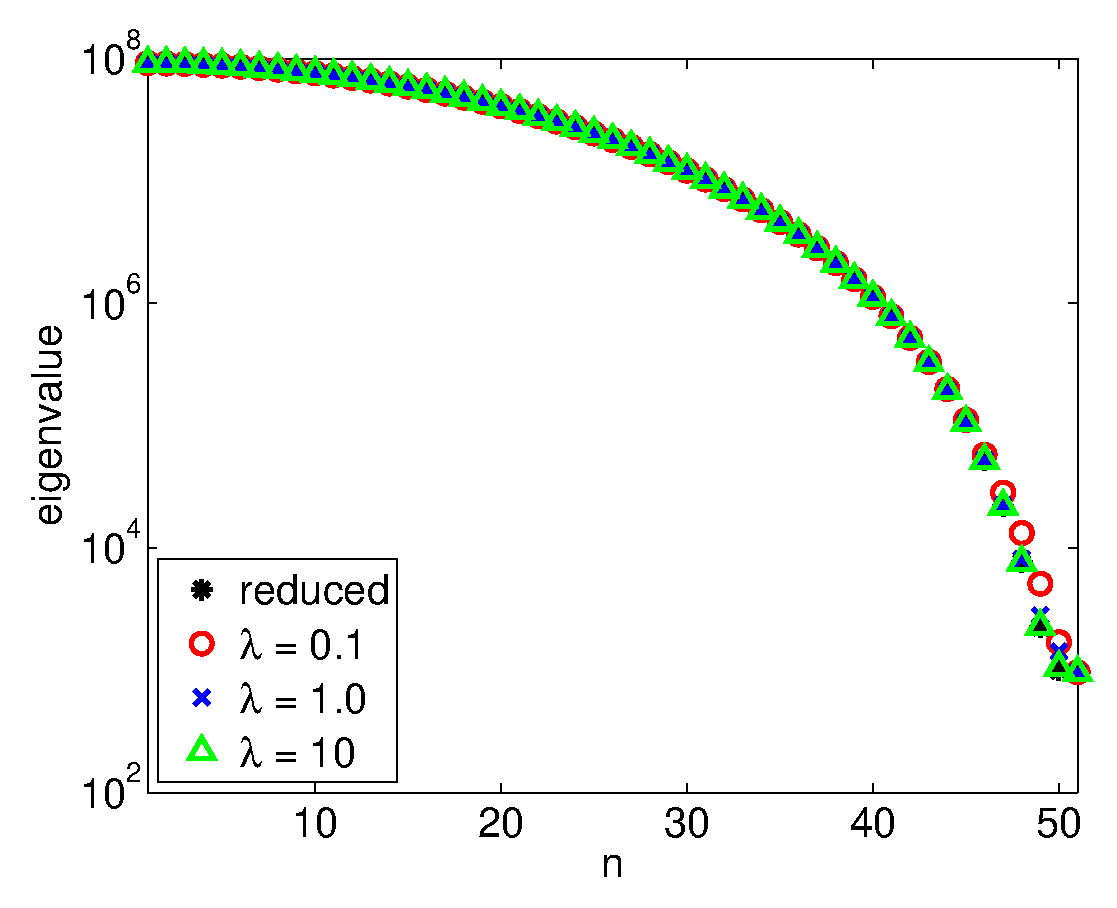
\includegraphics[scale=.2]{./figs/example2_a}&
\includegraphics[scale=.2]{./figs/example2_b}&
\includegraphics[scale=.2]{./figs/example2_c}\\
{\small $L = 1$}&{\small $L = 10$}&{\small $L = 20$}\\
\end{tabular}
\caption{Eigenvalues of the augmented system,  $A^TA + \lambda P_LP_L^T$, for various $\lambda$ and $L$, where $A$ is a finite-difference discritization of $\imath\omega - \partial_x\left(m(x)\partial_x\right)$
and $P_L$ is a restricted identify matrix of rank $L$. For comparison, the eigenvalues of the original system $A^TA$ are also shown.}
\label{fig:example2}
\end{figure}

\begin{figure}
\centering
\begin{tabular}{ccc}
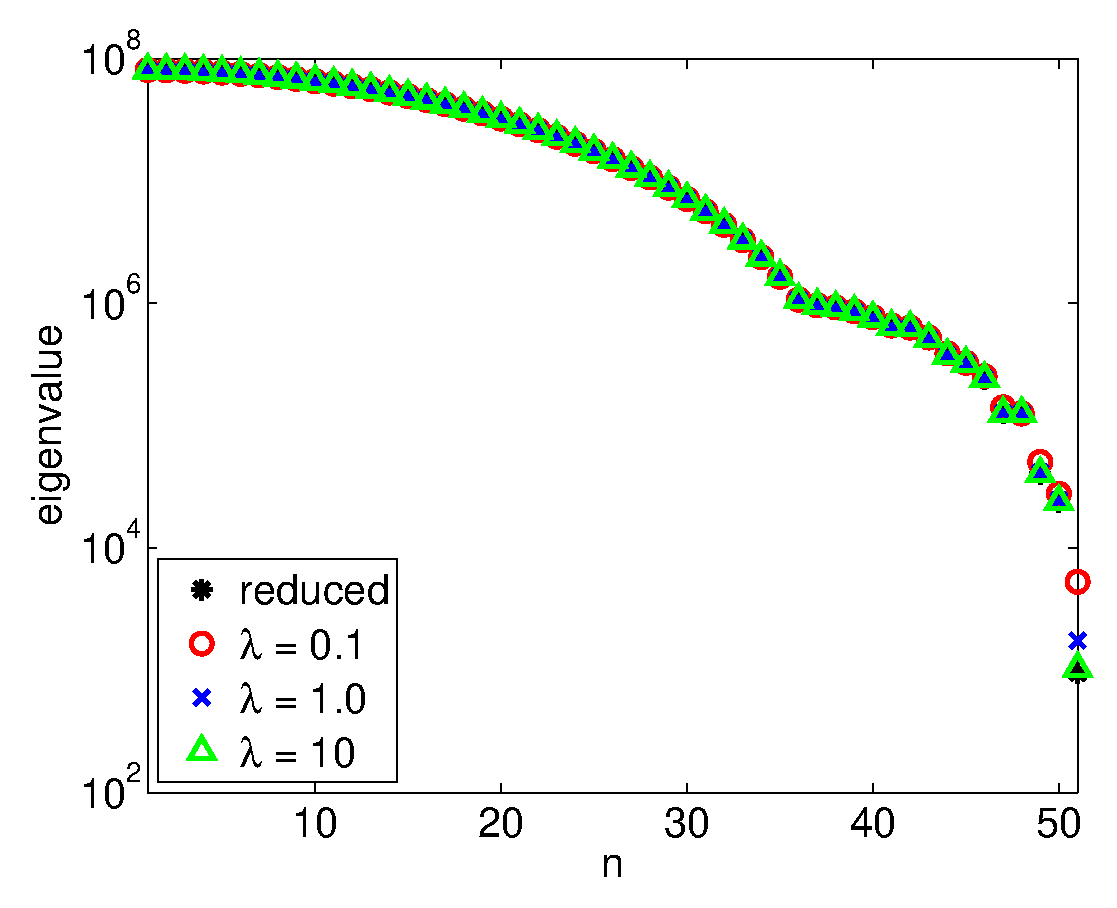
\includegraphics[scale=.2]{./figs/example3_a}&
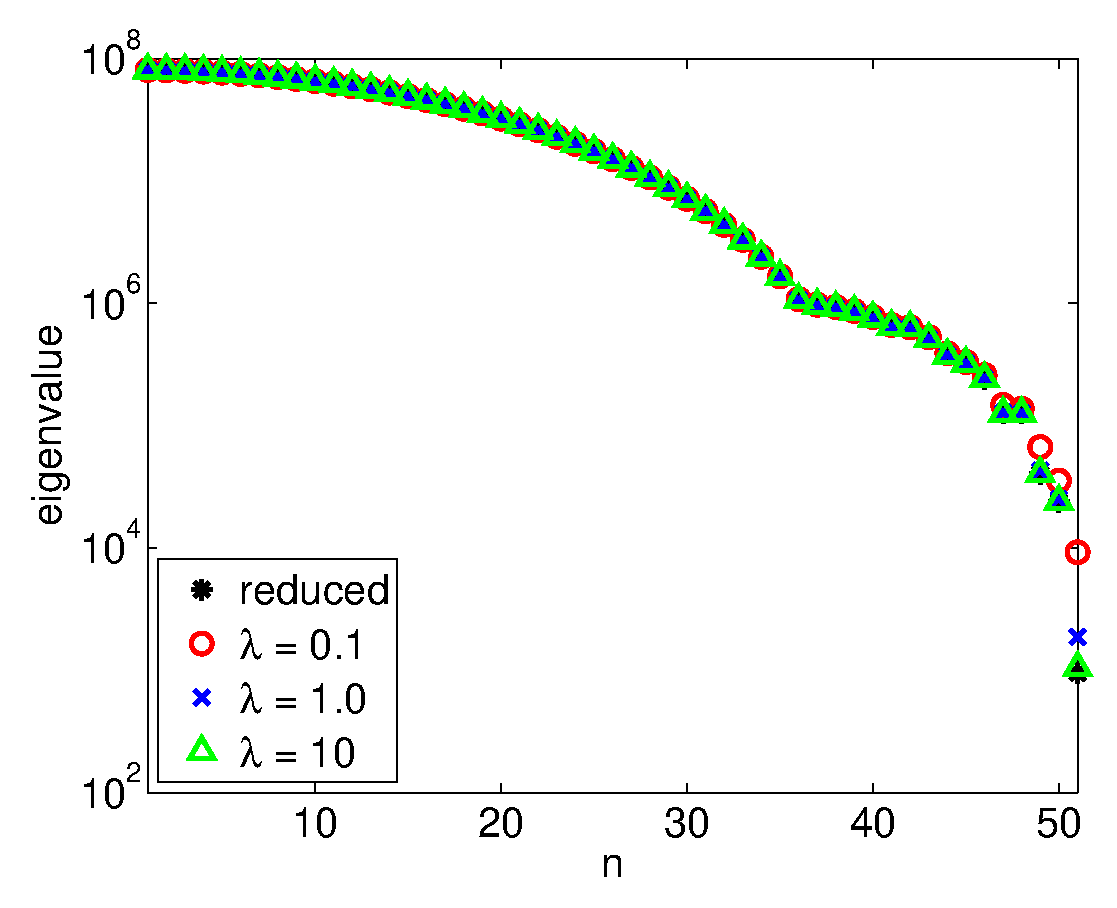
\includegraphics[scale=.2]{./figs/example3_b}&
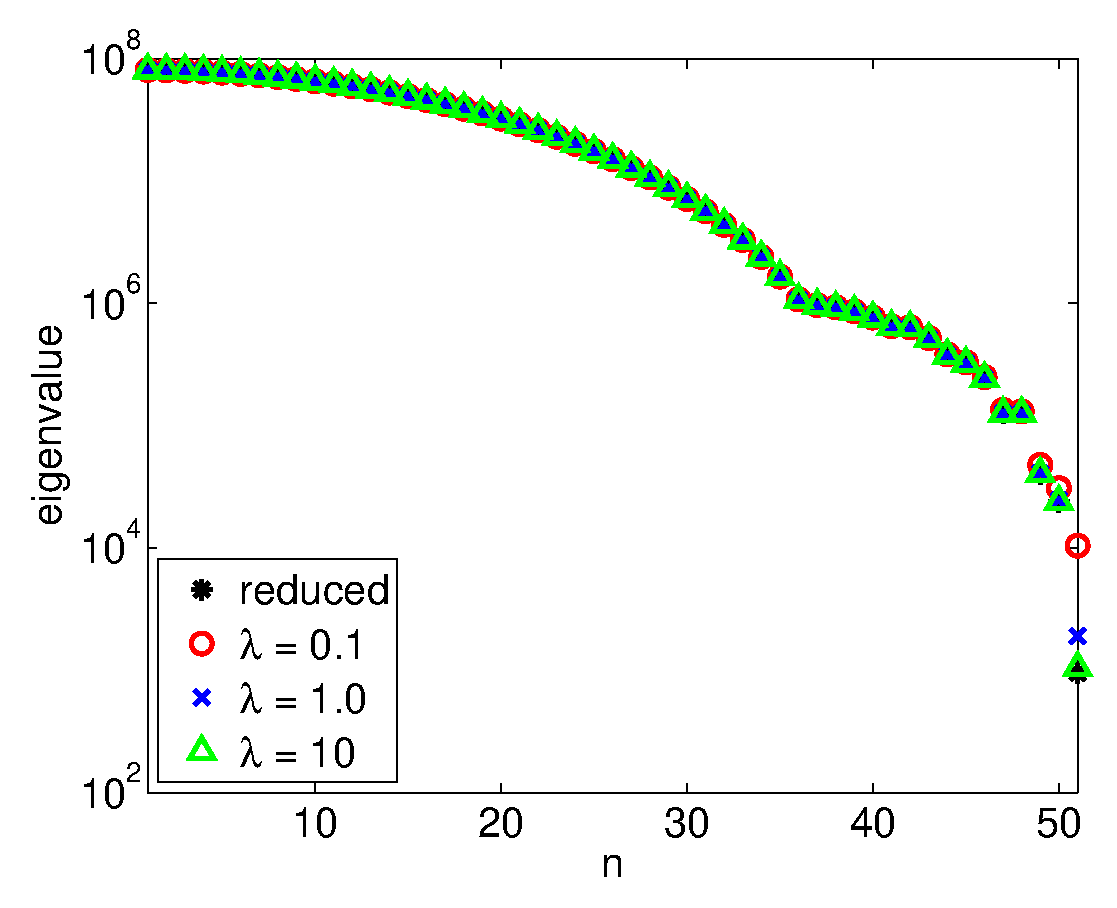
\includegraphics[scale=.2]{./figs/example3_c}\\
{\small $L = 1$}&{\small $L = 10$}&{\small $L = 20$}\\
\end{tabular}
\caption{Eigenvalues of the augmented system,  $A^TA + \lambda P_LP_L^T$, for various $\lambda$ and $L$, where $A$ is a finite-difference discritization of $\omega^2 + \partial_x^2$
and $P_L$ is a restricted identify matrix of rank $L$. For comparison, the eigenvalues of the original system $A^TA$ are also shown.}
\label{fig:example3}
\end{figure}

\begin{figure}
\centering
\begin{tabular}{cc}
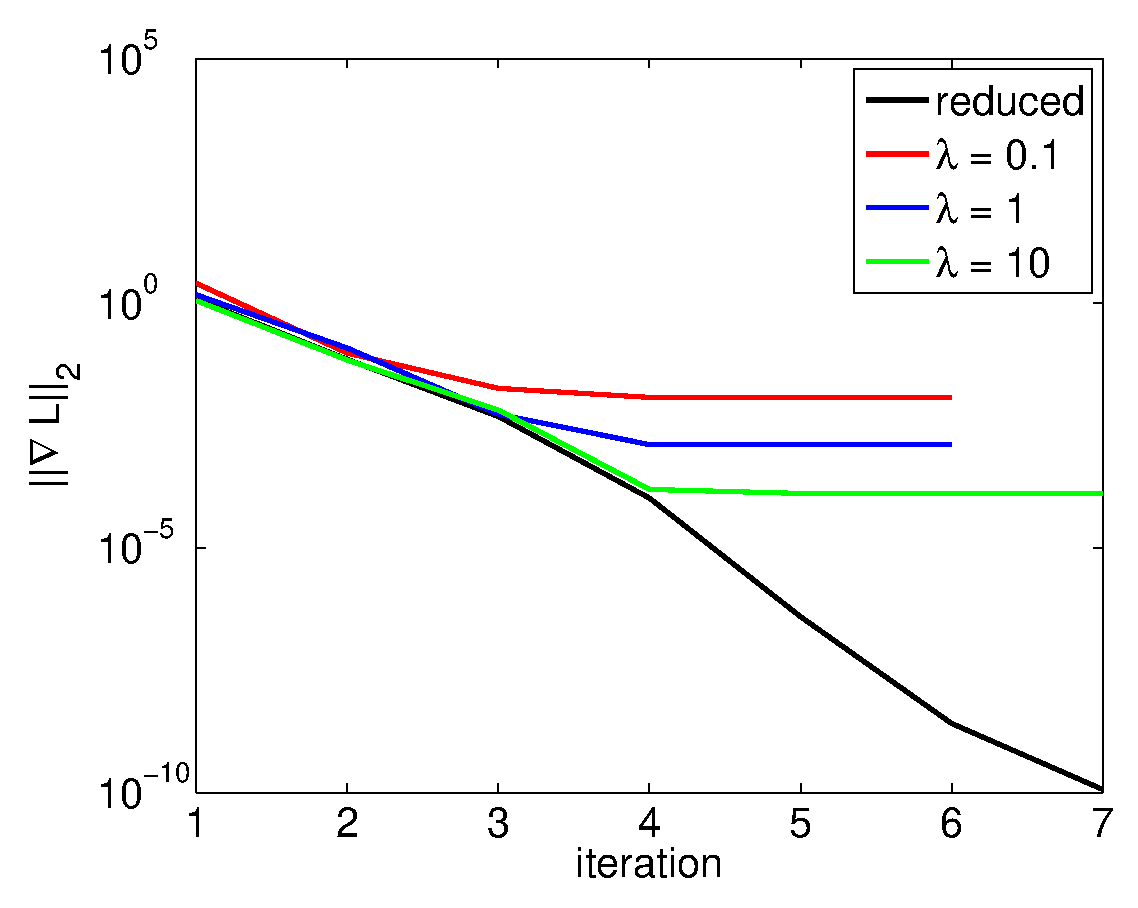
\includegraphics[scale=.4]{./figs/1D_exp1_a}&
\includegraphics[scale=.4]{./figs/1D_exp1_b}\\
{\small (a)}&{\small (b)}\\
\end{tabular}
\caption{Solutions and convergence history for 1D resisivity problem.}
\label{fig:1D_exp1}
\end{figure}

\begin{figure}
\centering
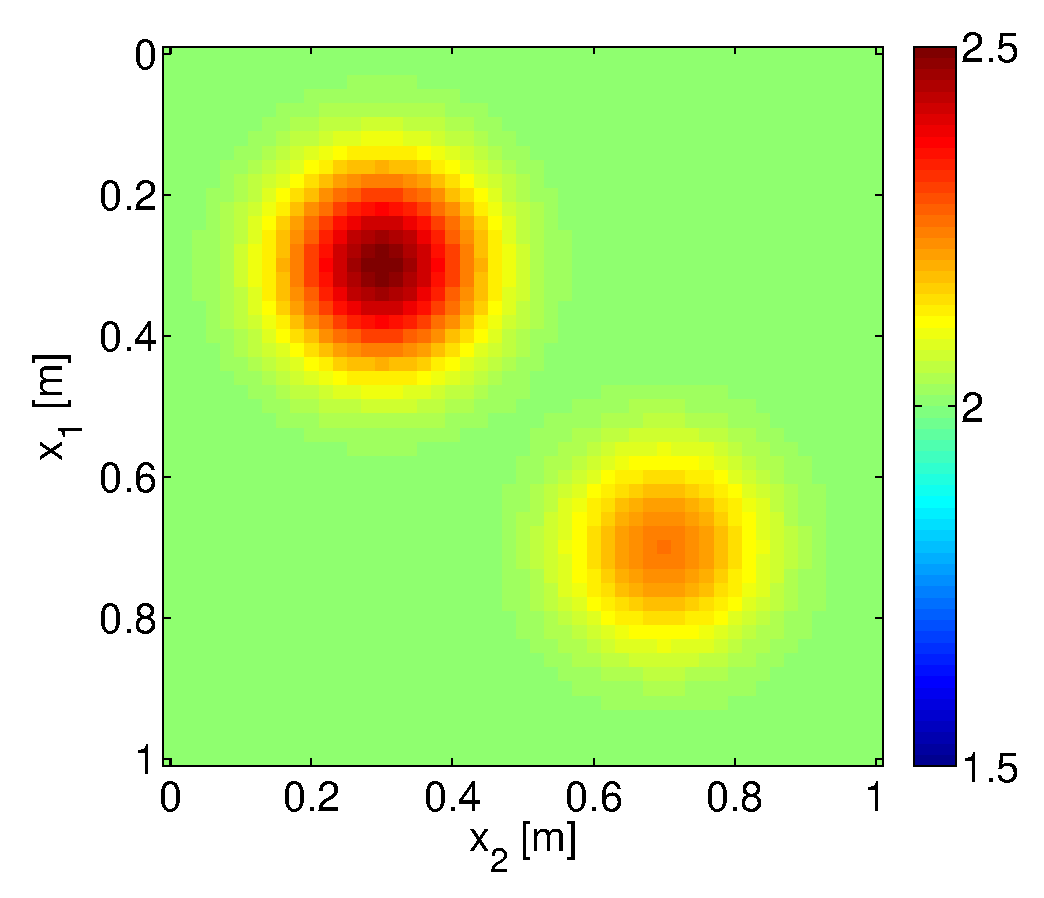
\includegraphics[scale=.4]{./figs/2D_exp1_a}\\
\caption{Ground truth model ($s^2/km^2$) and locations of the sources ($*$) and receivers ($\bigtriangledown$)}
\label{fig:2D_model}
\end{figure}

\begin{figure}
\centering
\begin{tabular}{cccc}
\includegraphics[scale=.2]{./figs/2D_exp0_a}&
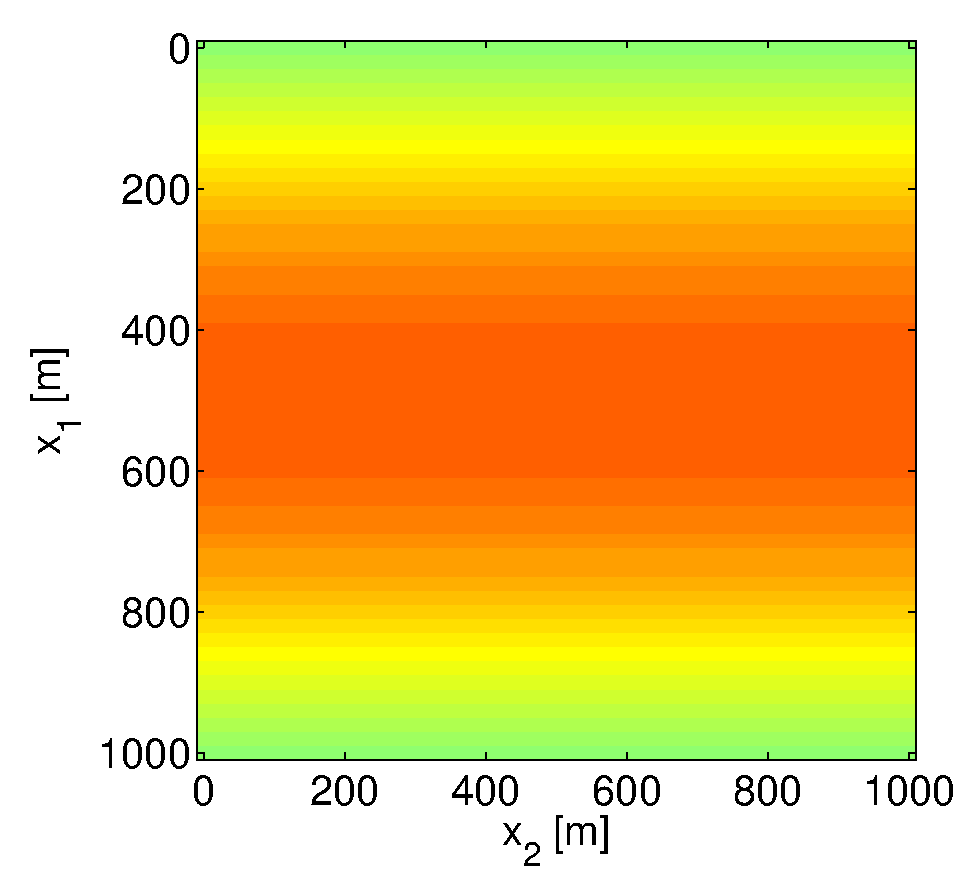
\includegraphics[scale=.2]{./figs/2D_exp0_b}&
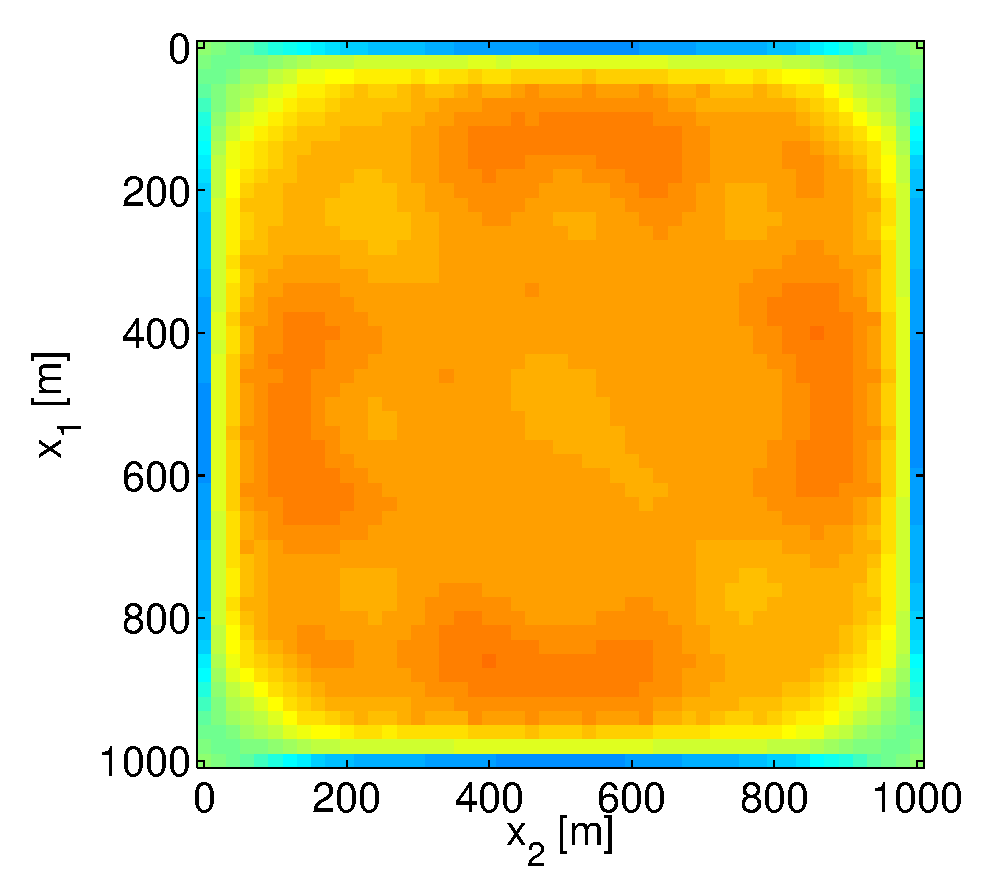
\includegraphics[scale=.2]{./figs/2D_exp0_c}&
\includegraphics[scale=.2]{./figs/2D_exp0_d}\\
\includegraphics[scale=.2]{./figs/2D_exp0_e}&
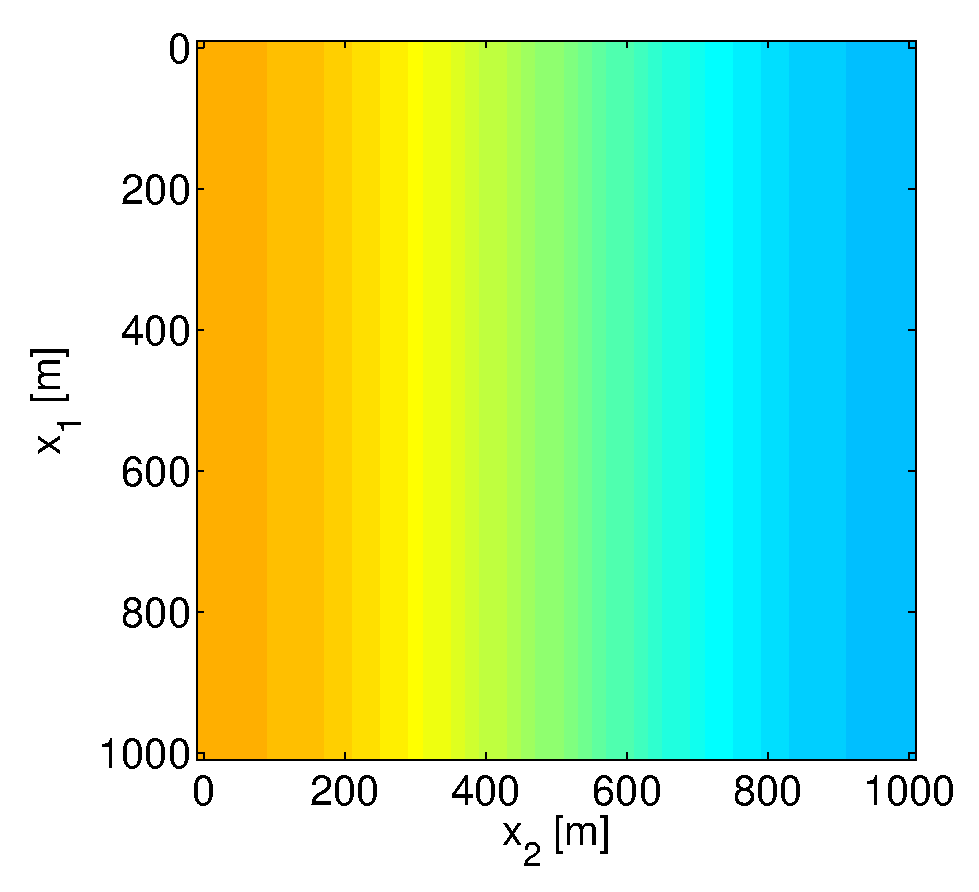
\includegraphics[scale=.2]{./figs/2D_exp0_f}&
\includegraphics[scale=.2]{./figs/2D_exp0_g}&
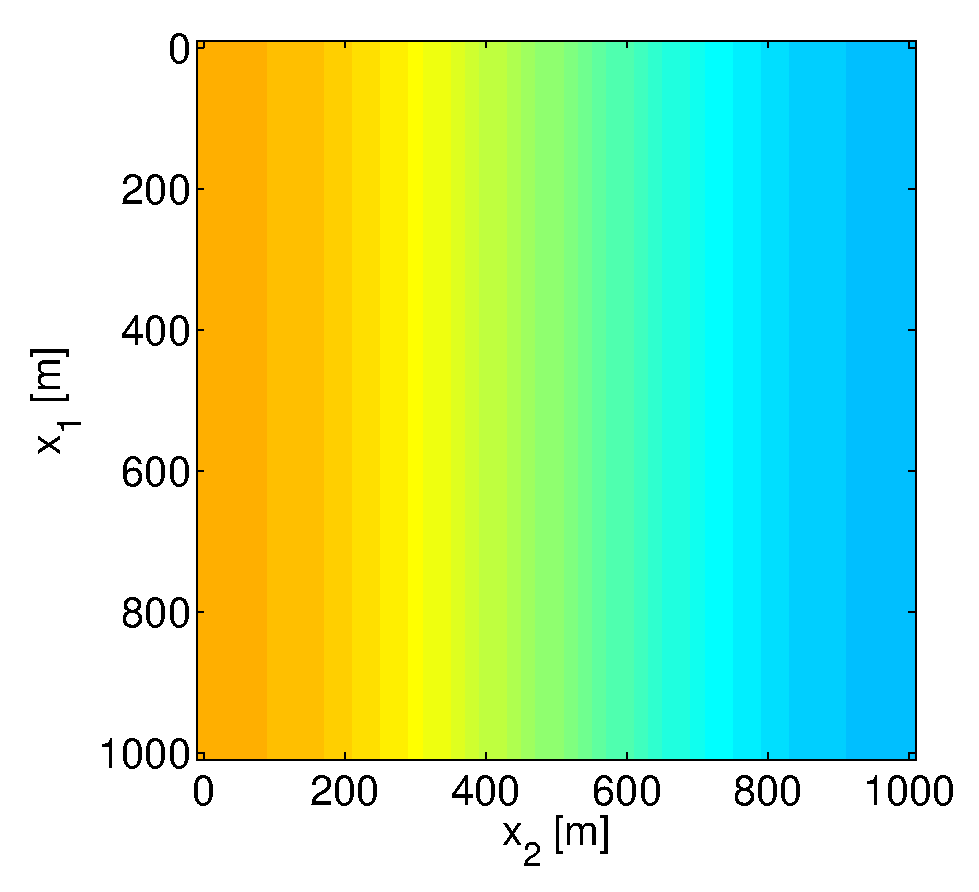
\includegraphics[scale=.2]{./figs/2D_exp0_h}\\
{\small reduced}&{\small $\lambda=0.1$}&{\small $\lambda=1$}&{\small $\lambda=10$}\\
\end{tabular}
\caption{Dominant eigenvectors of the GN Hessian.}
\label{fig:2D_exp0a}
\end{figure}

\begin{figure}
\centering
\begin{tabular}{cccc}
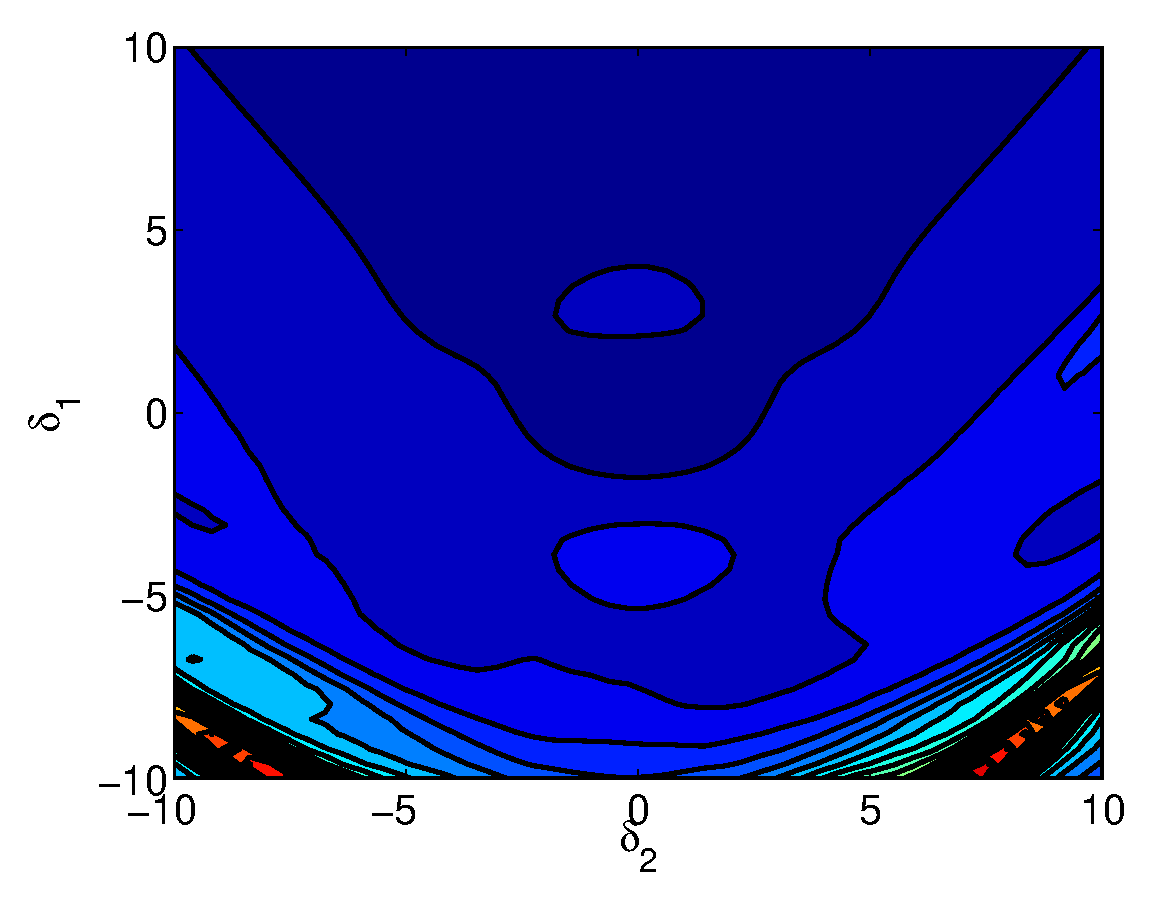
\includegraphics[scale=.2]{./figs/2D_exp0_i}&
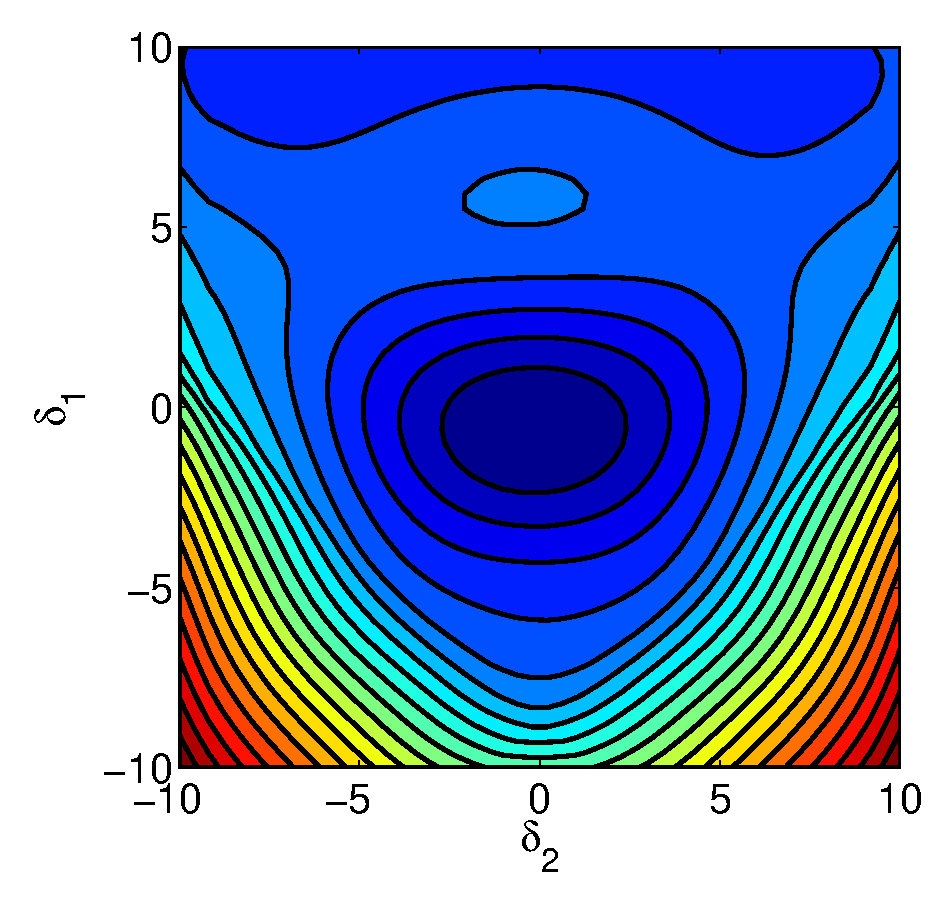
\includegraphics[scale=.2]{./figs/2D_exp0_j}&
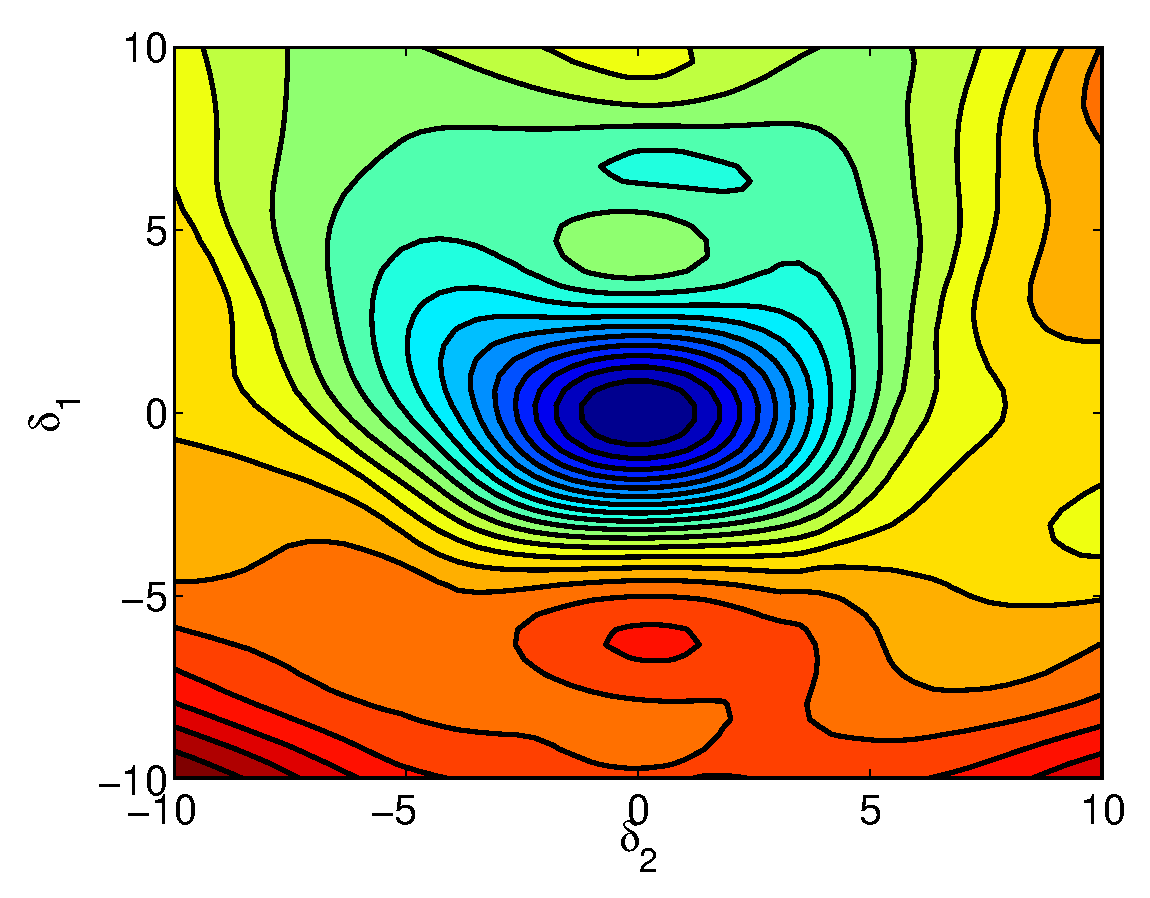
\includegraphics[scale=.2]{./figs/2D_exp0_k}&
\includegraphics[scale=.2]{./figs/2D_exp0_l}\\
{\small reduced}&{\small $\lambda=0.1$}&{\small $\lambda=1$}&{\small $\lambda=10$}\\
\end{tabular}
\caption{Misfit in the direction of the dominant eigenvector of the Hessian.}
\label{fig:2D_exp0b}
\end{figure}


\begin{figure}
\centering
\begin{tabular}{cc}
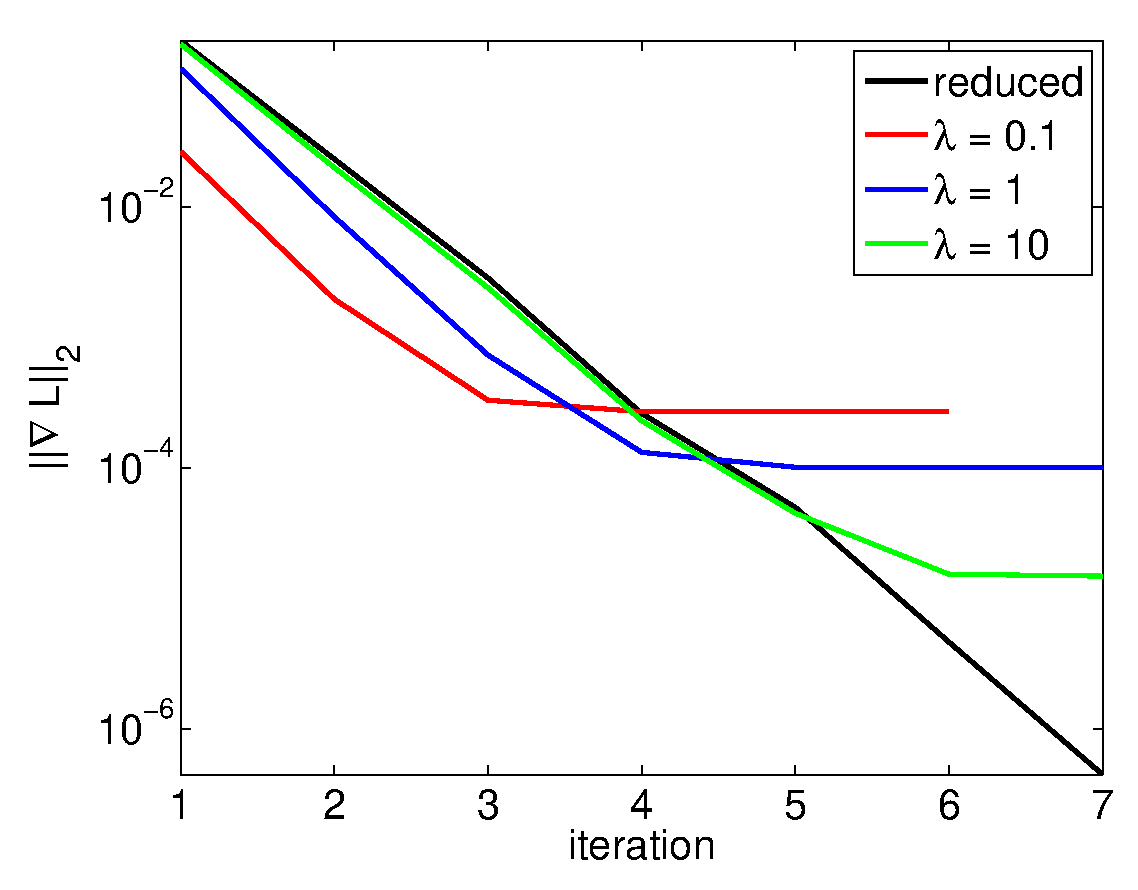
\includegraphics[scale=.3]{./figs/2D_exp1_b}&
\includegraphics[scale=.3]{./figs/2D_exp1_c}\\
\end{tabular}
\centering
\begin{tabular}{cccc}
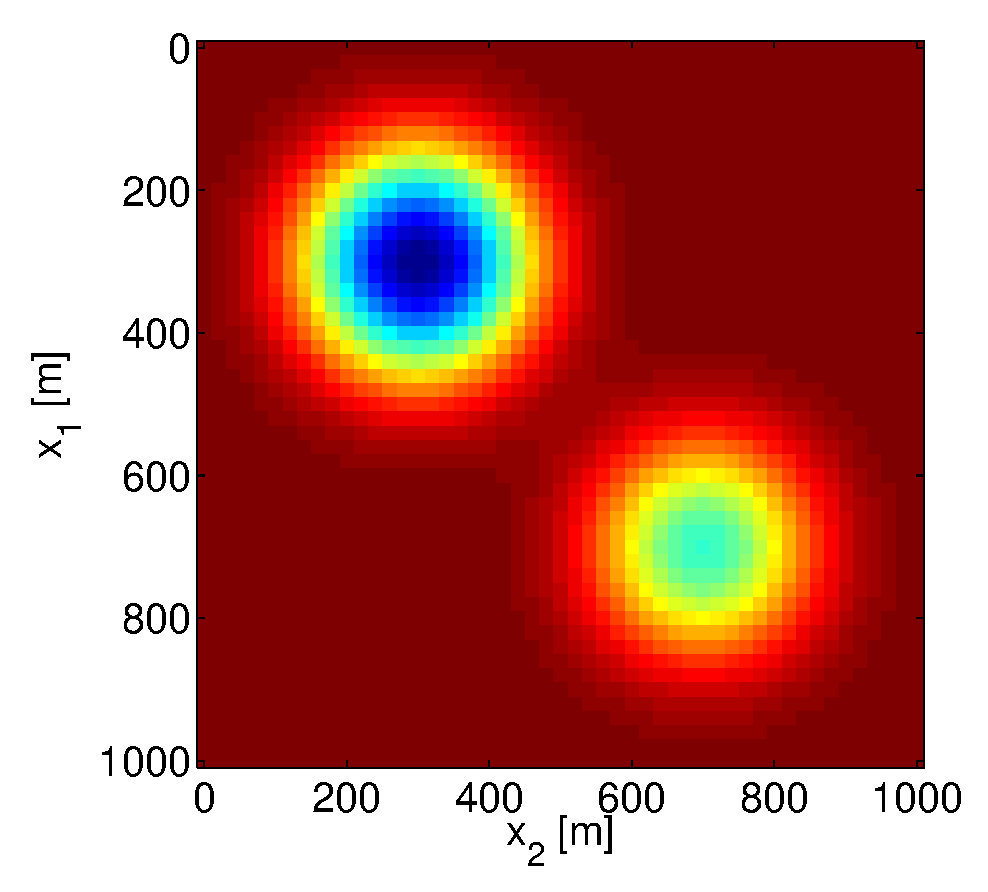
\includegraphics[scale=.2]{./figs/2D_exp1_d}&
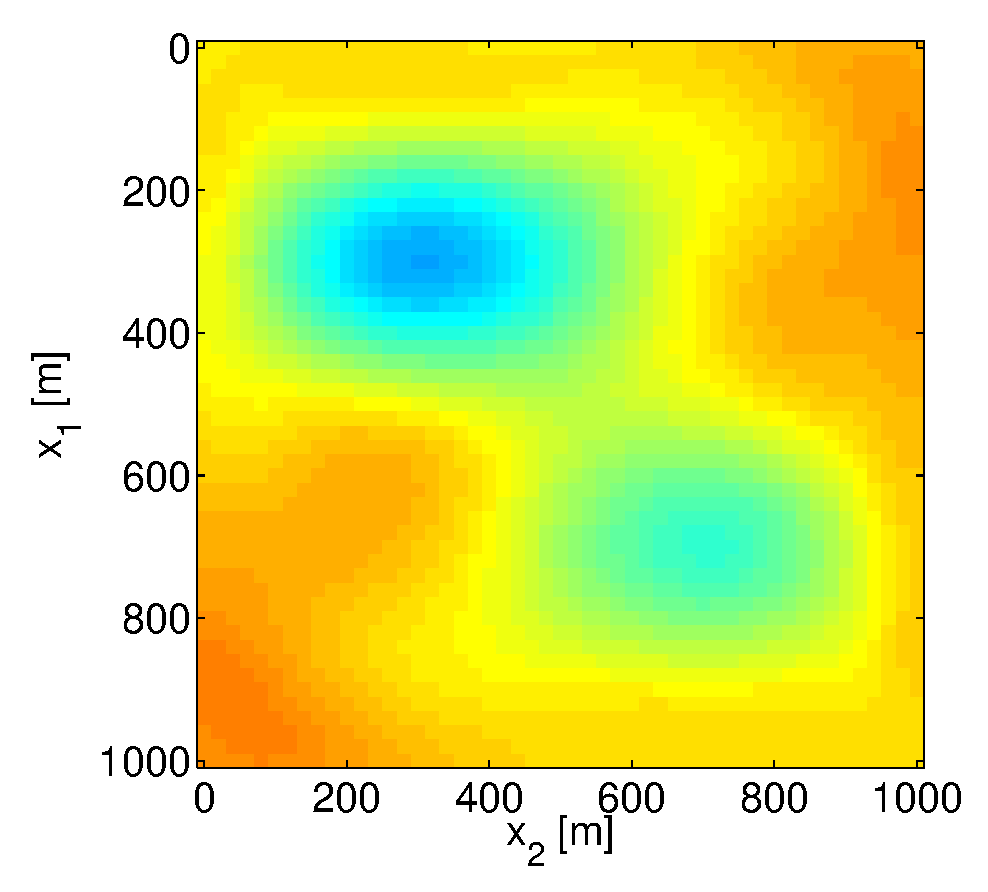
\includegraphics[scale=.2]{./figs/2D_exp1_e}&
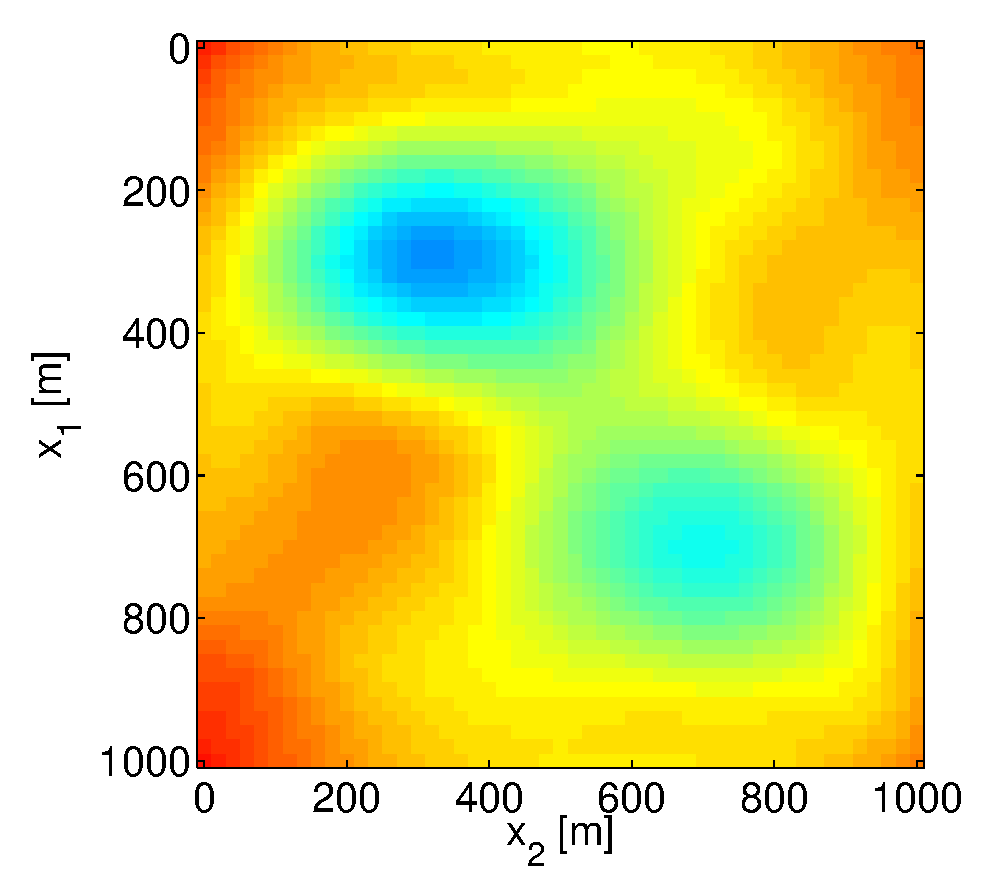
\includegraphics[scale=.2]{./figs/2D_exp1_f}&
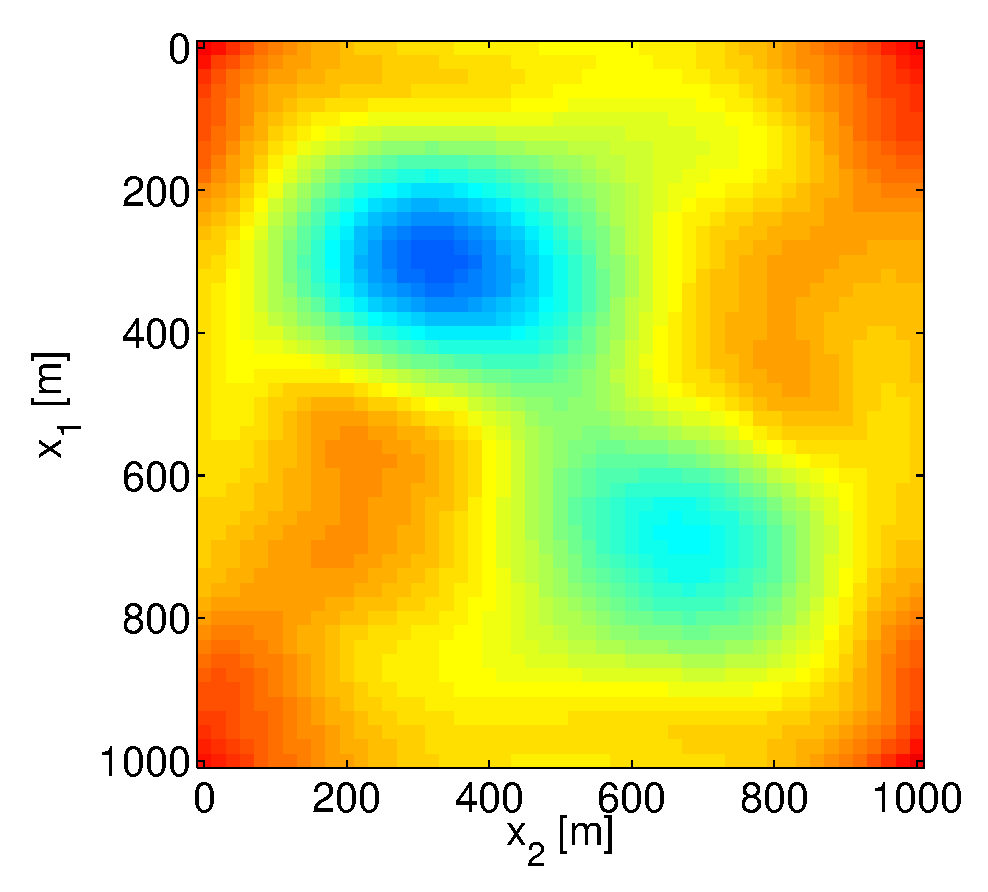
\includegraphics[scale=.2]{./figs/2D_exp1_g}\\
{\small reduced}&{\small $\lambda=0.1$}&{\small $\lambda=1$}&{\small $\lambda=10$}\\
\end{tabular}
\caption{Convergence history, GN reconstruction error and reconstructions for data without noise.}
\label{fig:2D_exp1}
\end{figure}

\begin{figure}
\centering
\begin{tabular}{cc}
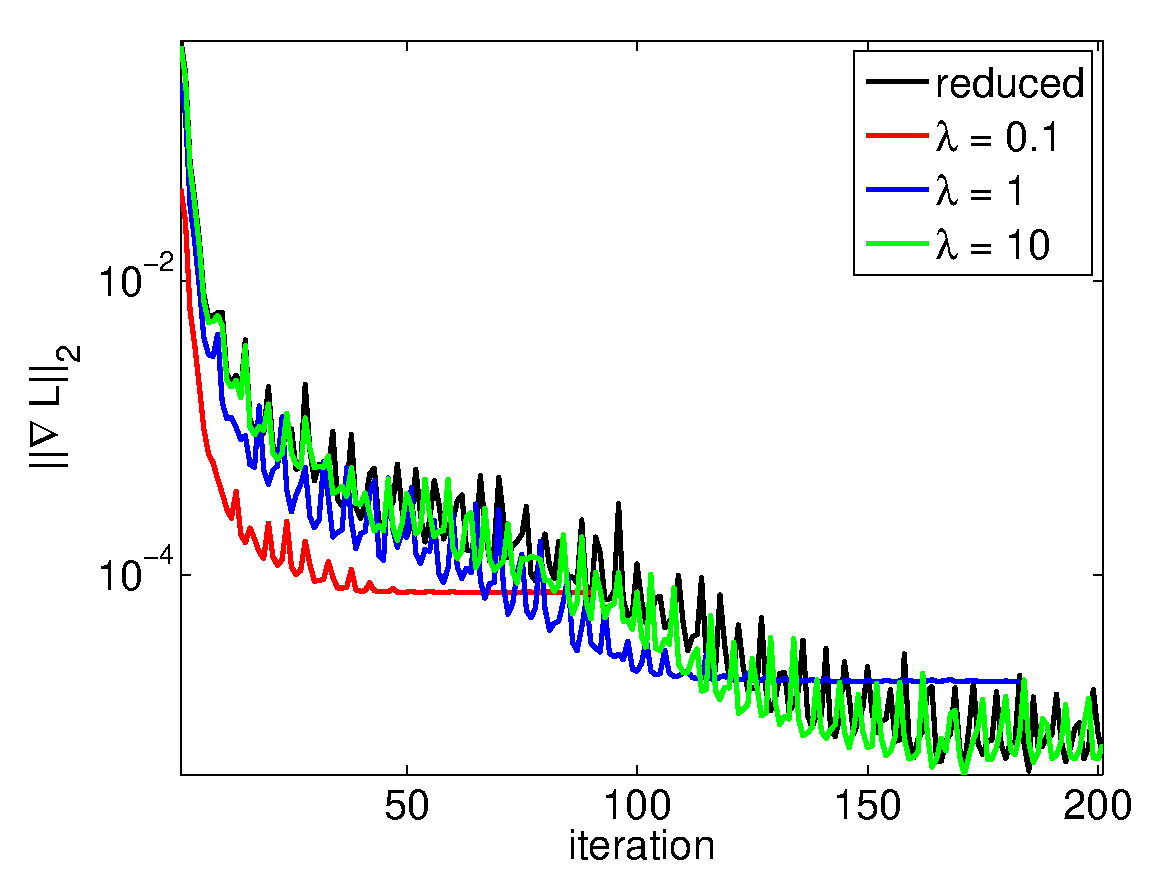
\includegraphics[scale=.3]{./figs/2D_exp2_b}&
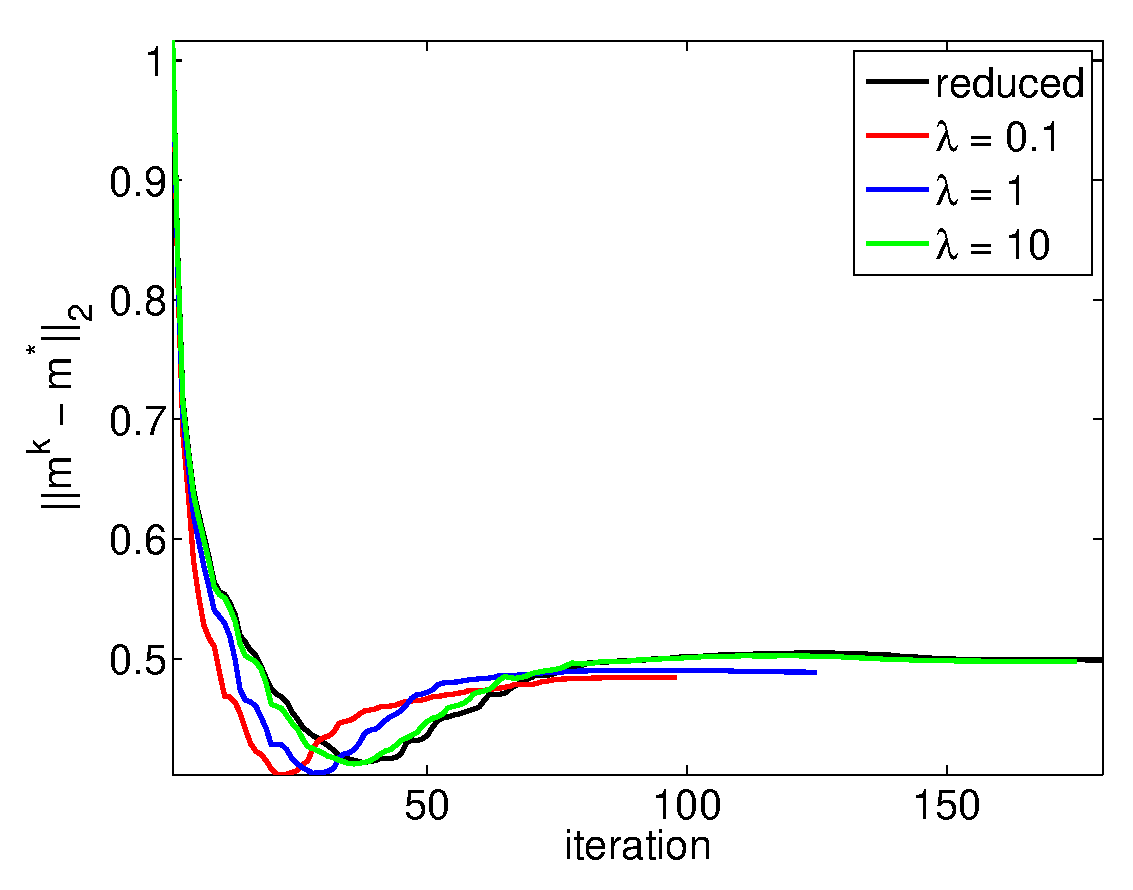
\includegraphics[scale=.3]{./figs/2D_exp2_c}\\
\end{tabular}
\centering
\begin{tabular}{cccc}
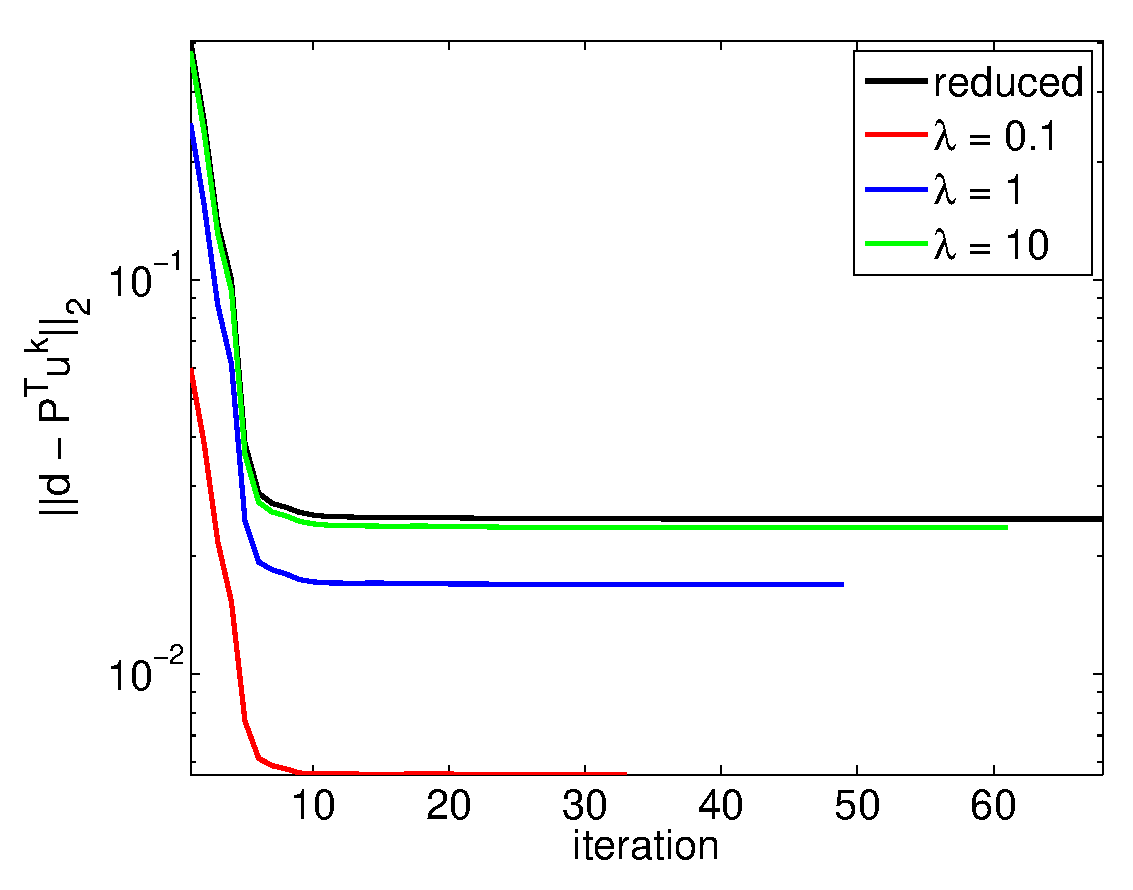
\includegraphics[scale=.2]{./figs/2D_exp2_d}&
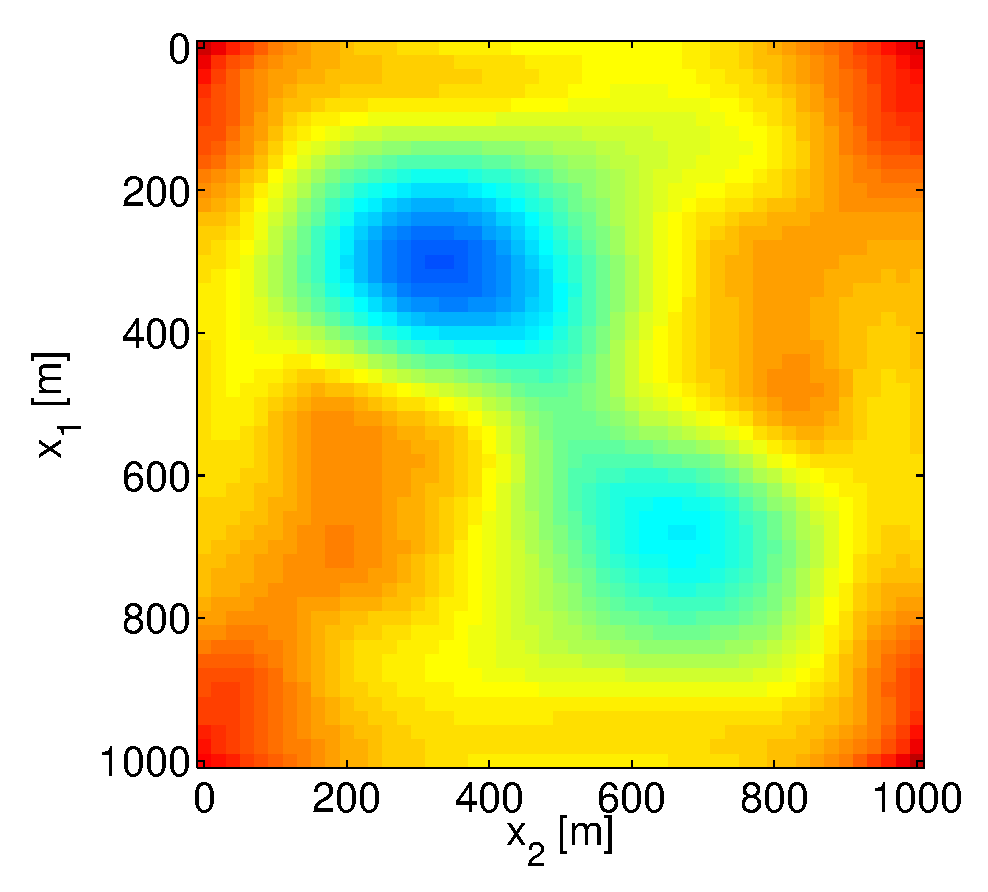
\includegraphics[scale=.2]{./figs/2D_exp2_e}&
\includegraphics[scale=.2]{./figs/2D_exp2_f}&
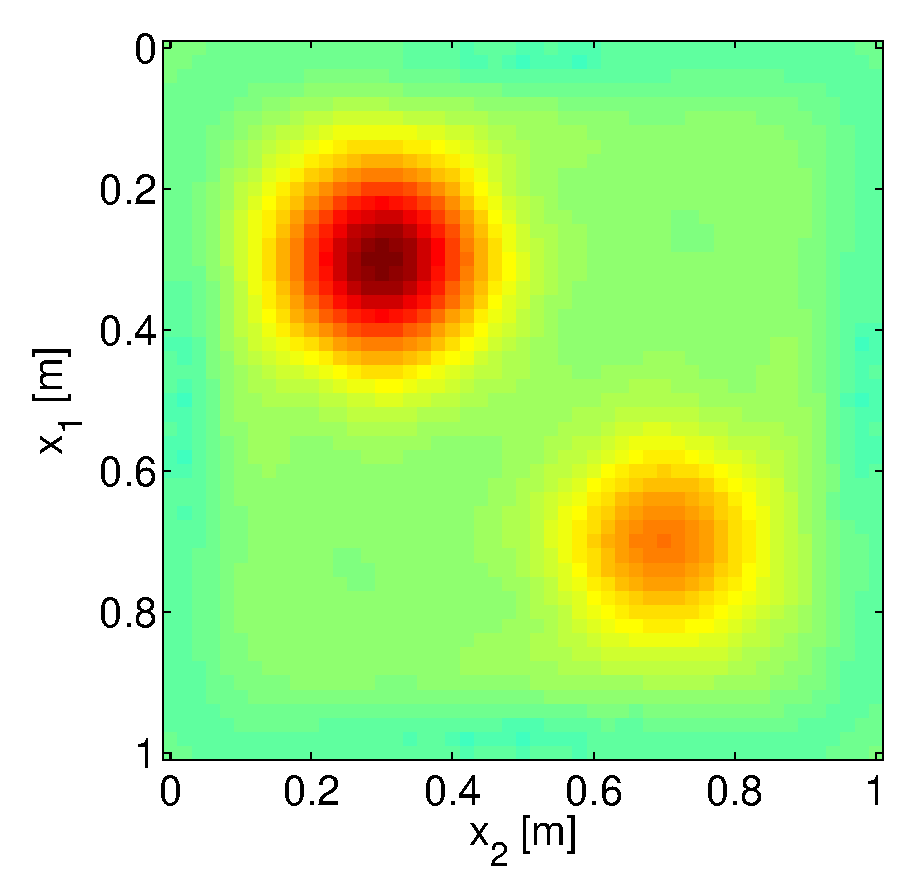
\includegraphics[scale=.2]{./figs/2D_exp2_g}\\
{\small reduced}&{\small $\lambda=0.1$}&{\small $\lambda=1$}&{\small $\lambda=10$}\\
\end{tabular}
\caption{Convergence history, QN reconstruction error and reconstructions for data without noise.}
\label{fig:2D_exp2}
\end{figure}

\begin{figure}
\centering
\begin{tabular}{cc}
\includegraphics[scale=.3]{./figs/2D_exp3_b}&
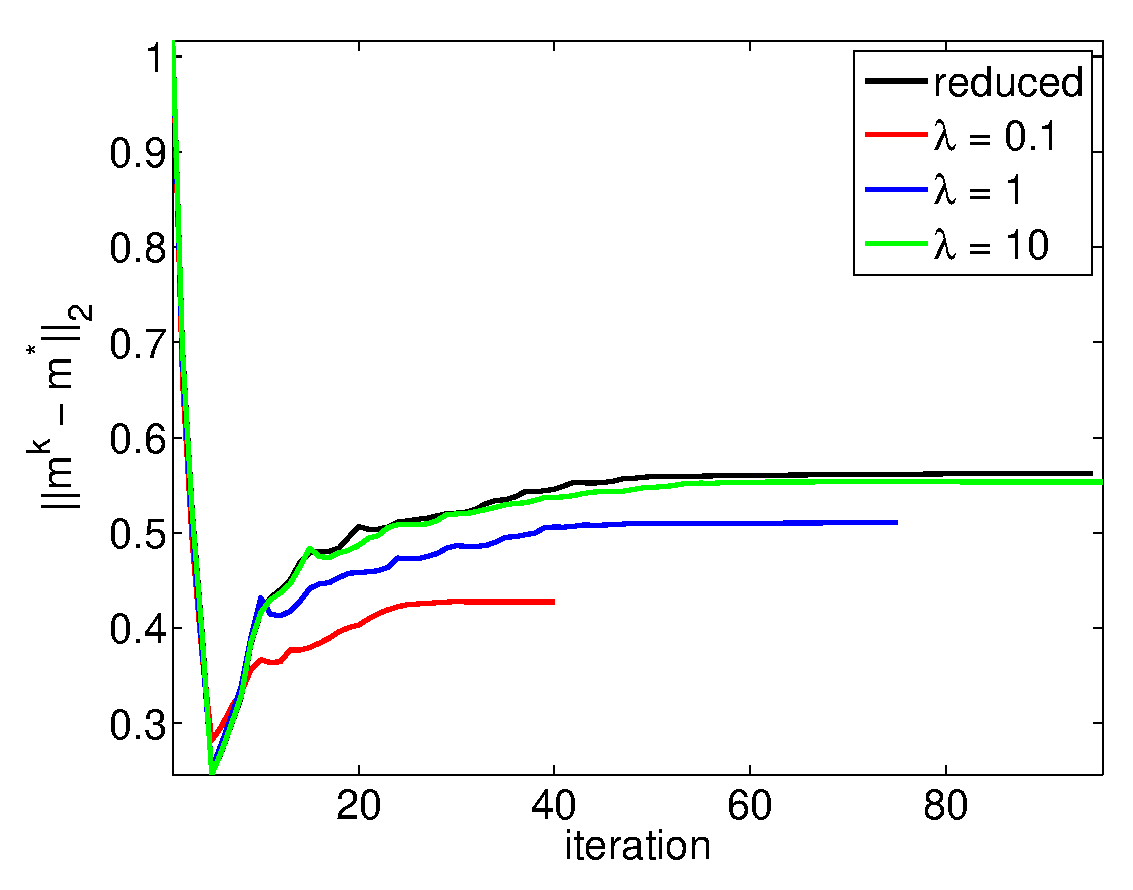
\includegraphics[scale=.3]{./figs/2D_exp3_c}\\
\end{tabular}
\centering
\begin{tabular}{cccc}
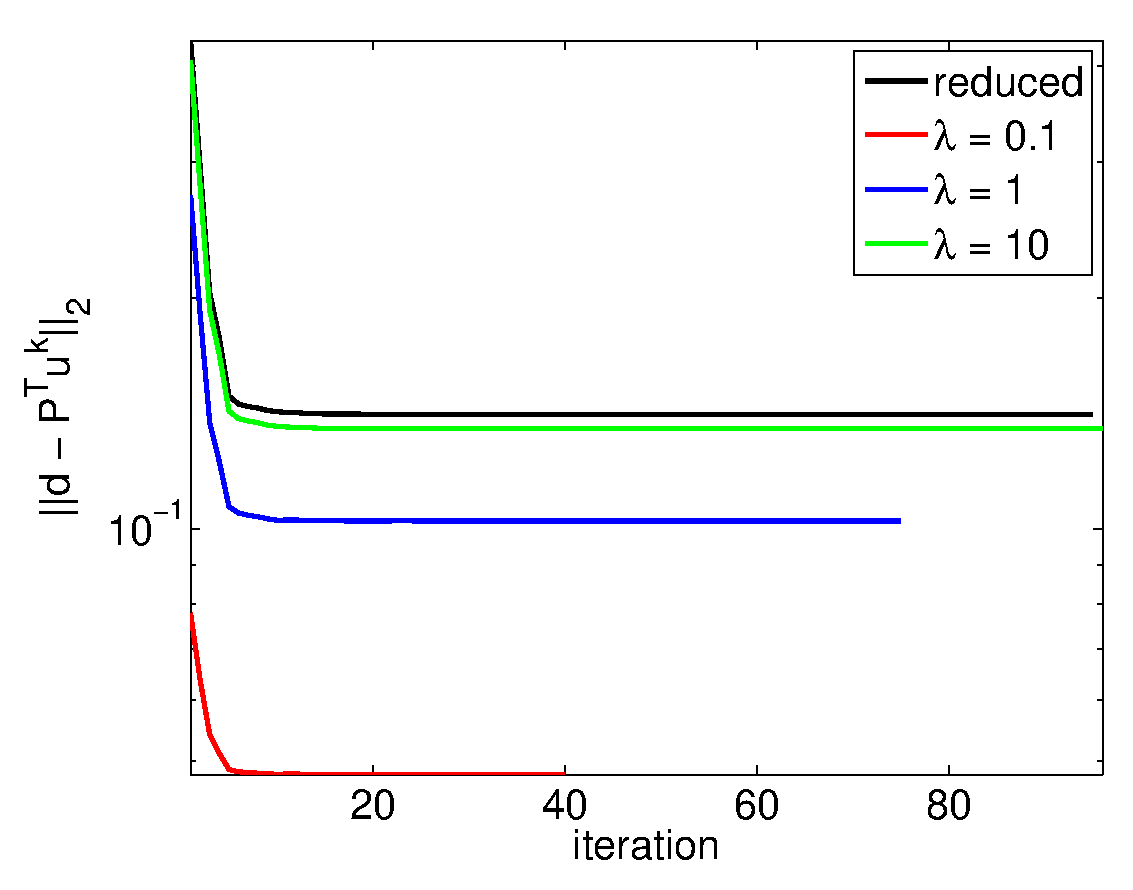
\includegraphics[scale=.2]{./figs/2D_exp3_d}&
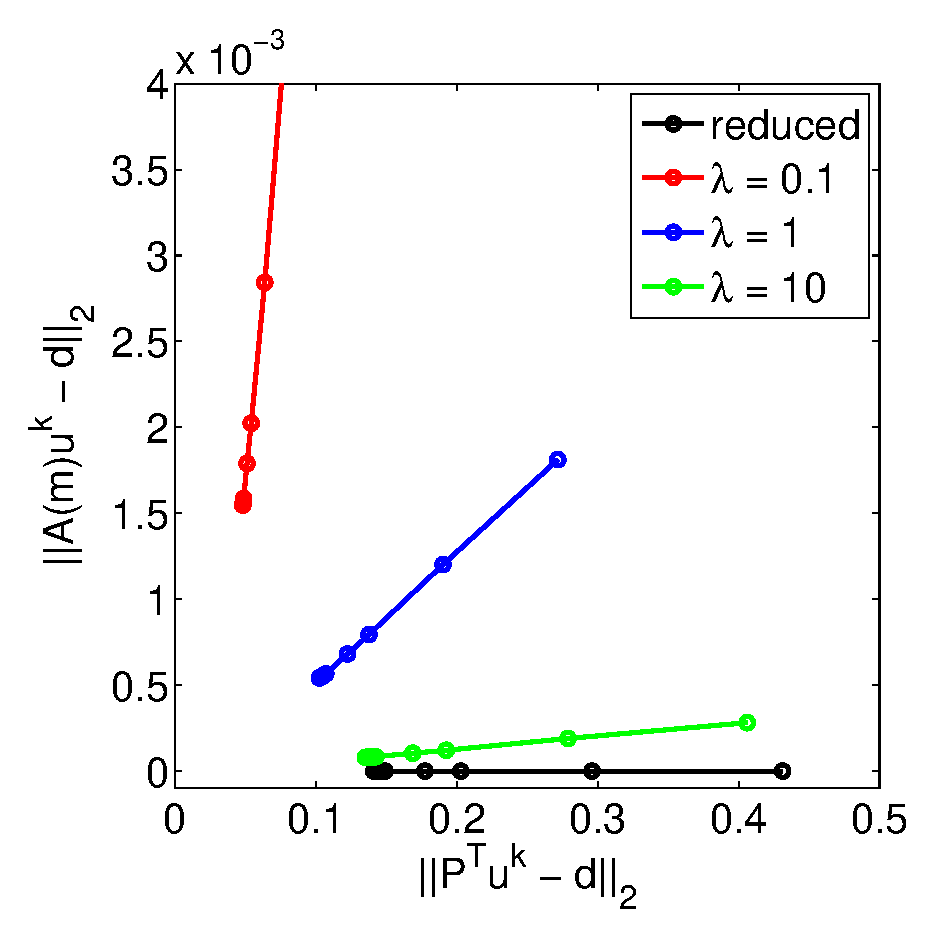
\includegraphics[scale=.2]{./figs/2D_exp3_e}&
\includegraphics[scale=.2]{./figs/2D_exp3_f}&
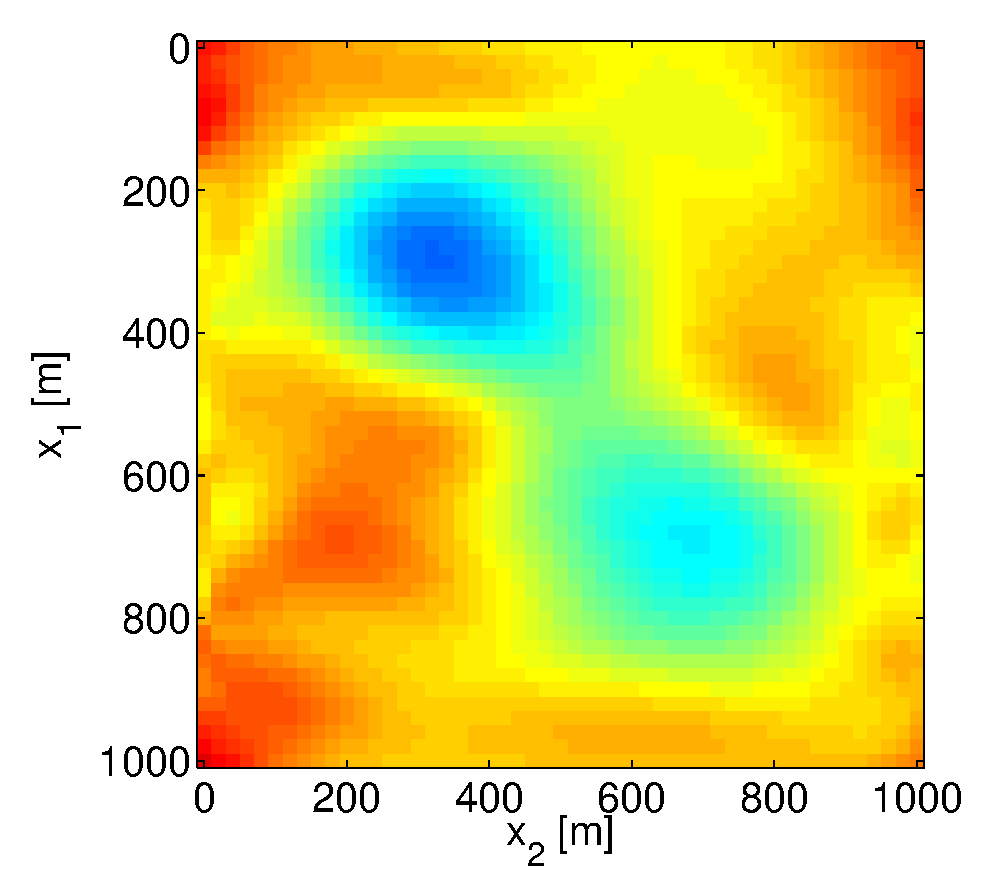
\includegraphics[scale=.2]{./figs/2D_exp3_g}\\
{\small reduced}&{\small $\lambda=0.1$}&{\small $\lambda=1$}&{\small $\lambda=10$}\\
\end{tabular}
\caption{Convergence history, QN reconstruction error and reconstructions for data with 10\% Gaussian noise.}
\label{fig:2D_exp3}
\end{figure}

\begin{figure}
\centering
\begin{tabular}{cc}
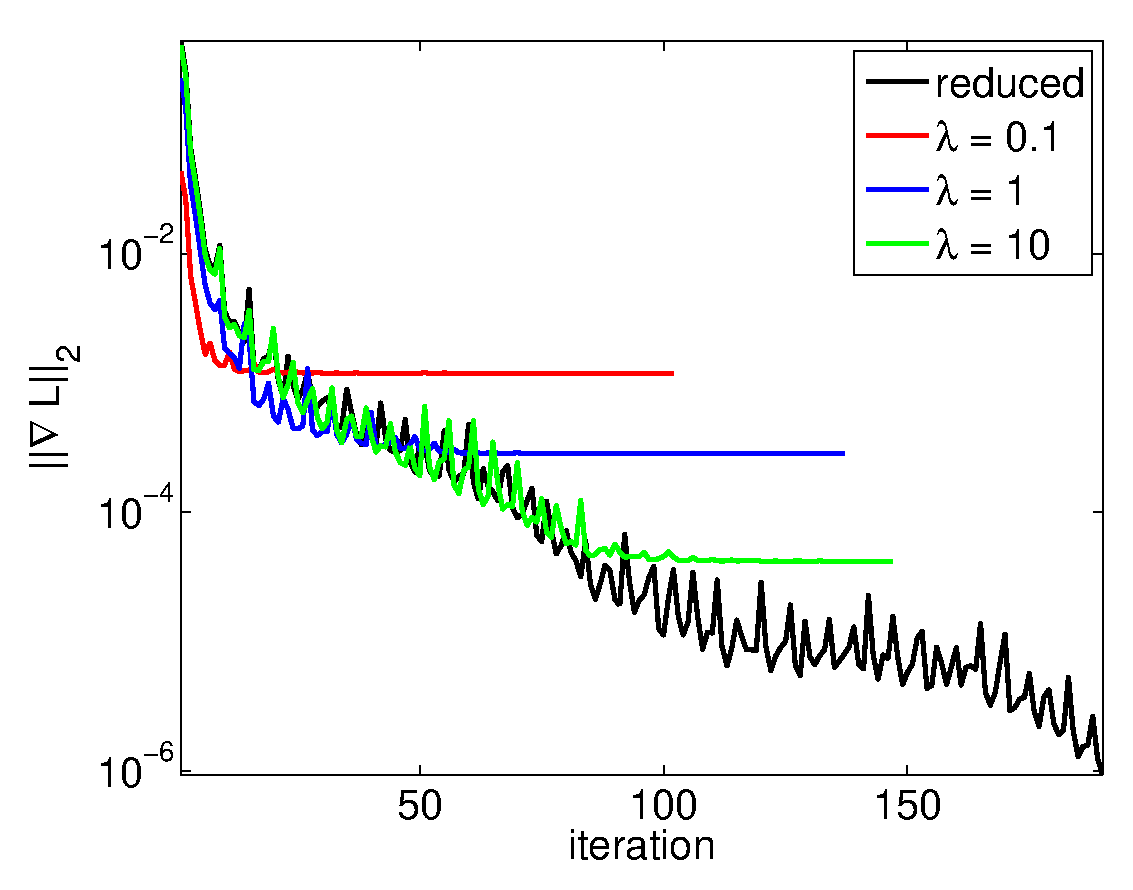
\includegraphics[scale=.3]{./figs/2D_exp4_b}&
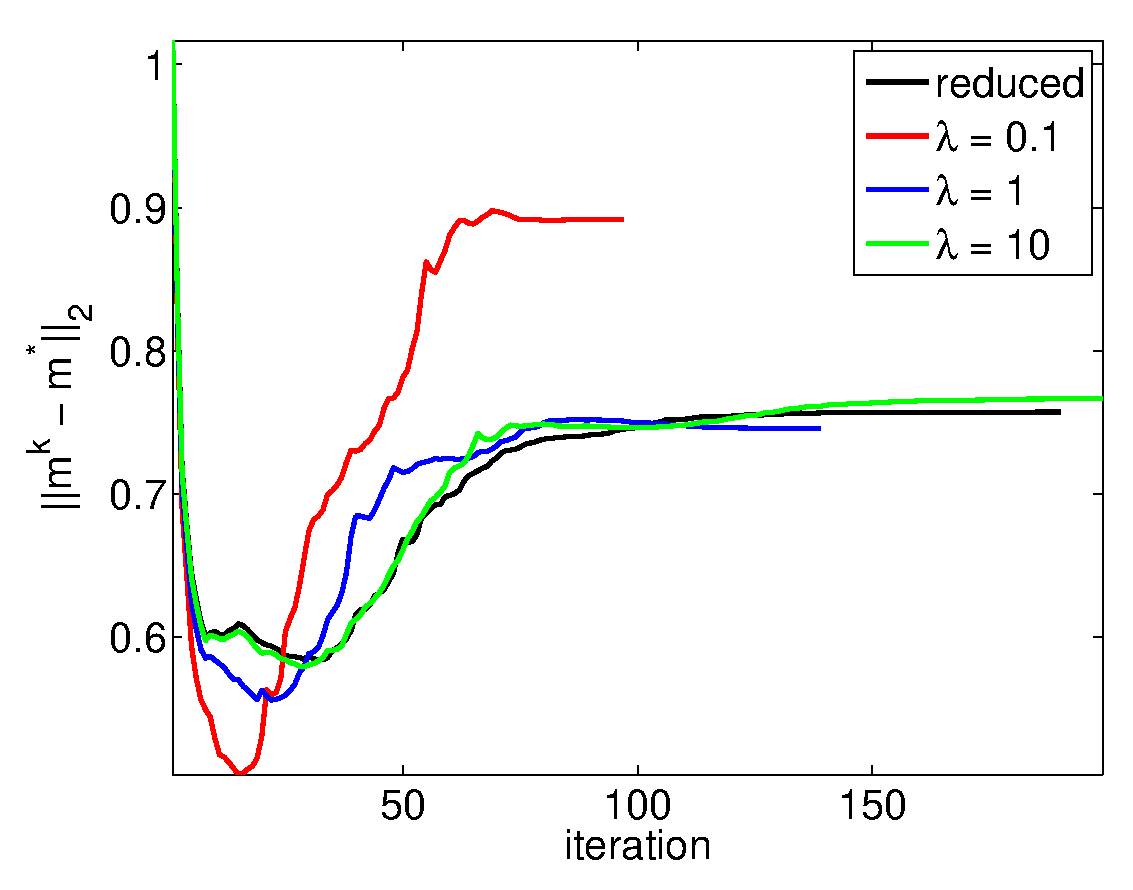
\includegraphics[scale=.3]{./figs/2D_exp4_c}\\
\end{tabular}
\centering
\begin{tabular}{cccc}
\includegraphics[scale=.2]{./figs/2D_exp4_d}&
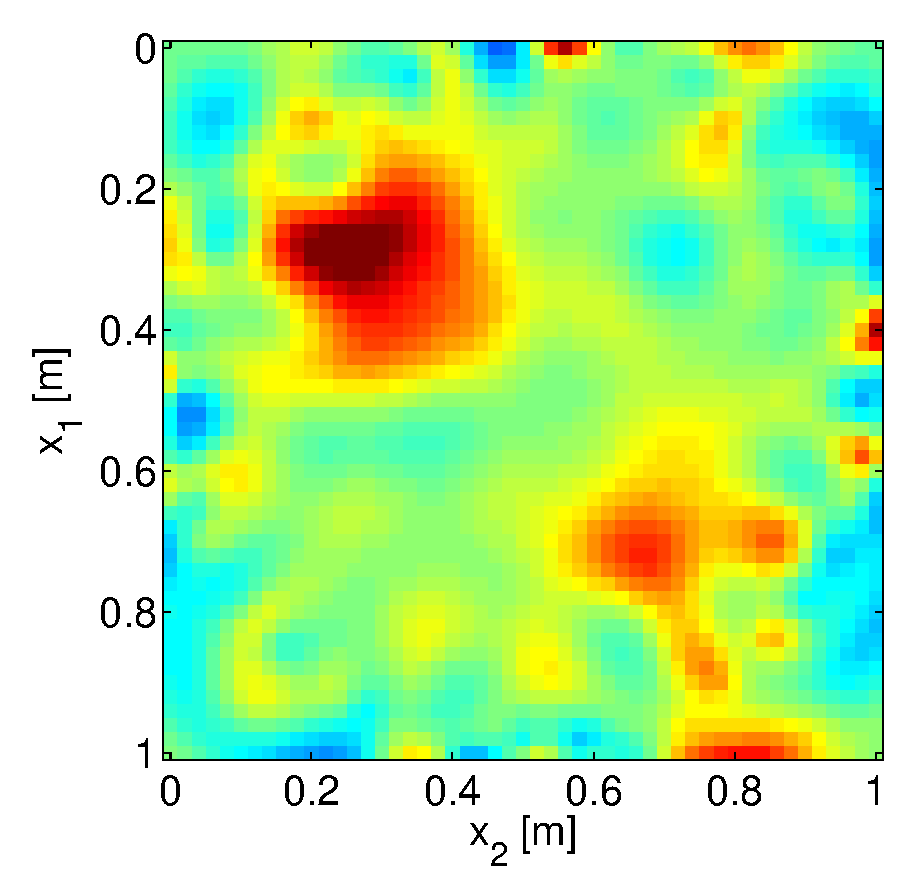
\includegraphics[scale=.2]{./figs/2D_exp4_e}&
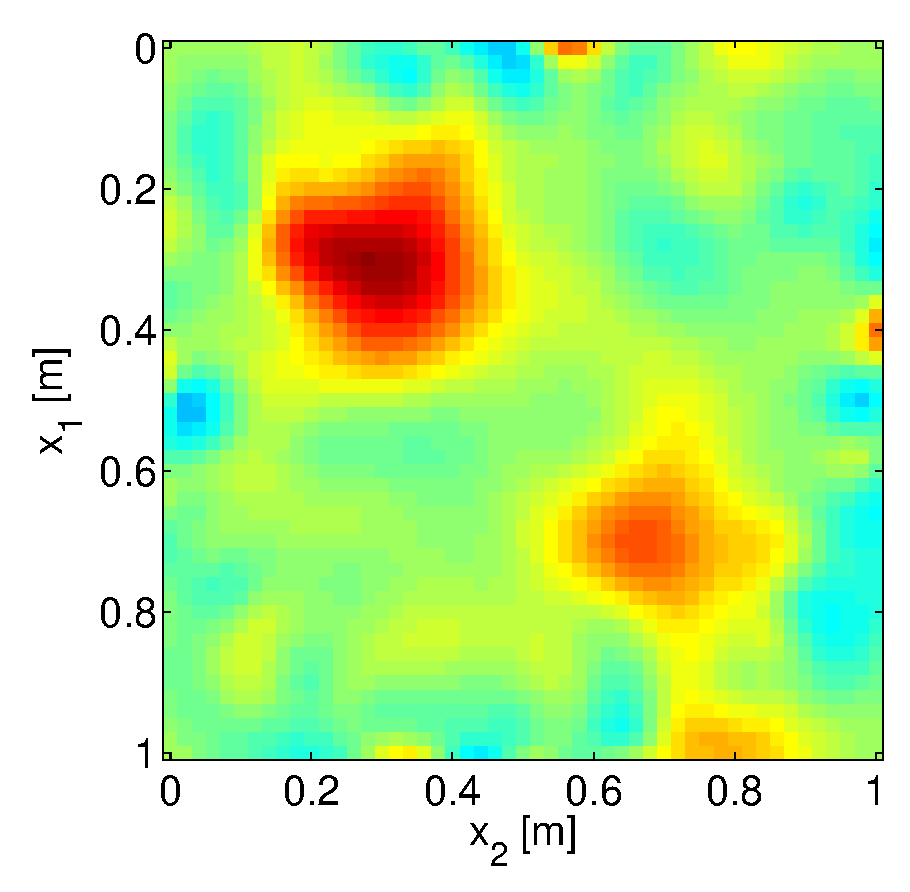
\includegraphics[scale=.2]{./figs/2D_exp4_f}&
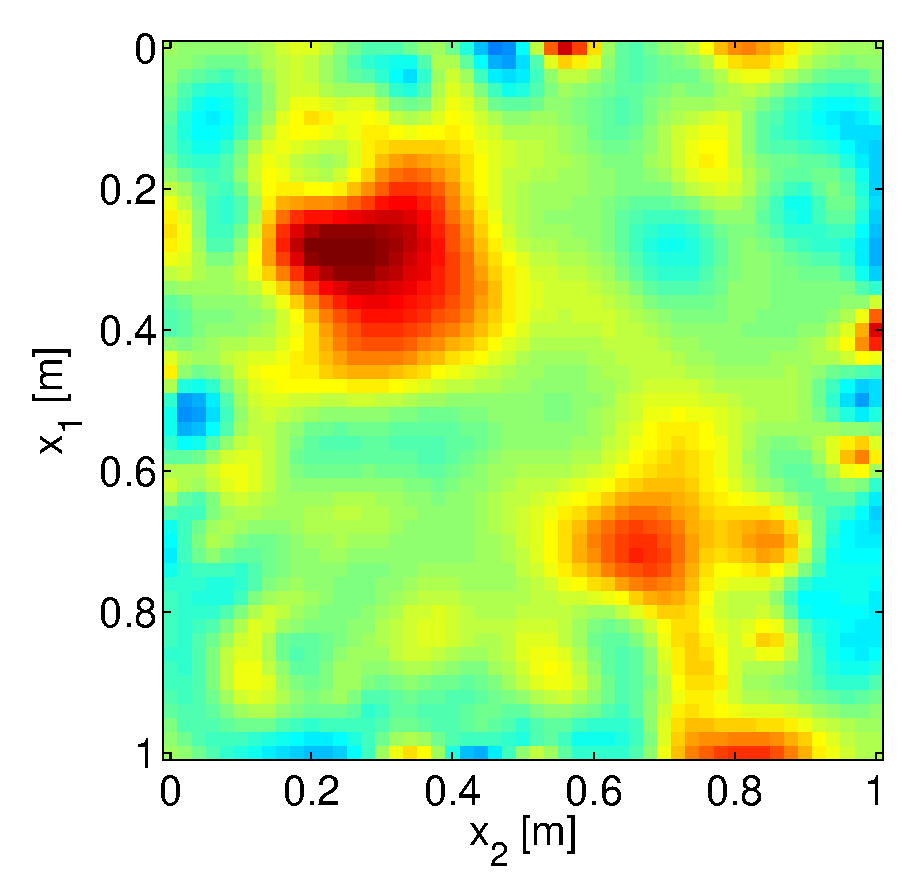
\includegraphics[scale=.2]{./figs/2D_exp4_g}\\
{\small reduced}&{\small $\lambda=0.1$}&{\small $\lambda=1$}&{\small $\lambda=10$}\\
\end{tabular}
\caption{Convergence history, QN reconstruction error and reconstructions for data with 20\% Gaussian noise.}
\label{fig:2D_exp3}
\end{figure}

\clearpage
\bibliographystyle{unsrt}
\bibliography{mybib}



\end{document}

